%! suppress = MissingImport
\subsection*{Abstract}
\label{subsec:ni-abs}

Non-interference\index{non-interference} is an information flow
policy\index{information flow!policy} for guaranteeing \ndx{confidentiality},
\ie that effects of sensitive data are not exposed to lower-level users, even
indirectly. When phrased in terms of programming languages, non-interference is
studied by attaching \ndx{security class}es to variables, then analyzing the
classes to determine if a violation, or a data \enquote{\ndx{leak}}, can occur.
Security type systems\index{security type system} are common controls for
analyzing and enforcing \ndx{non-interference}. Unfortunately, they require
inference algorithms, program-level security \ndx{specifications}, non-standard
compilers, and are generally too restrictive or complex for practical
implementation. In this paper, we present a program logic \lname that guarantees
the semantic security property of \emph{anytime
non-interference}\index{non-interference!anytime}. By anytime, we mean a
malicious actor with low-level access cannot infer anything about higher-level
values at any point of the program execution. The logic links
\ndx{non-interference} violations precisely to the faulty commands and
violations cannot be erased by program composition. We draw rich inspiration
from complexity-theoretic flow calculi, but obtaining a logic for security
analysis required significant adjustments. Finally, we share a prototype to
demonstrate \lname can be implemented as an automatic, annotation-free, static
security analyzer to obtain confidentiality guarantees in practice.

\subsection{Introduction}
\label{subsec:ni-introduction}

Verifying that data is handled securely during computation is challenging
because it requires information beyond the program syntax. For example, consider
a hash function that computes a checksum of its input. Assume there exists a
malicious actor who can observe outputs of the hash function. If all inputs are
public data, we can guarantee the function does not expose secrets to the actor.
However, if we change the inputs to secret data, like social security numbers,
we no longer have the same guarantee for the same function. The hash function
then \enquote{\ndx{leak}s} information that possibly enables
the actor to recover the secret data.

\emph{Non-interference}~\cite{goguen1982}\index{non-interference} is a classical
semantic security property that constrains \ndx{information flow} during
computation. It is a mechanism to enforce \emph{\ndx{confidentiality}}, \ie
concealment of information or resources from unauthorized
parties~\cite{bishop2003}. Non-interference\index{non-interference} is an
attractive target of study because it offers strong end-to-end guarantees for
data protection, it is inherently compositional\index{compositionality}, and can
be enforced with program logics or \ndx{security type
system}s~\cite{cecchetti2017,frumin2021}. Informally, a program is
non-interfering when secret data does not affect calculation of its public
outputs~\cite{sabelfeld2003}. In other words, data can only stay at the same
\ndx{security class} or flow to higher classes. Although a desirable property,
\ndx{non-interference} is in general undecidable by \ndx{Rice's
Theorem}~\cite{rice1953} and constructing a system that completely adheres to
\ndx{non-interference} is overly restrictive to capture real-world security
requirements~\cite{bossi2005,cecchetti2017}. However, unattainability of an
ideal construction does not restrict analysis of imperfect systems. Program
analysis enables detecting \ndx{information flow} issues, supports informed
assessments of vulnerabilities, and identifies potential mitigations.

Our work extends the analysis of \ndx{non-interference} in theoretical
directions while yielding practical advantages. In literature, terminology
around \ndx{non-interference} is defined somewhat fluidly~\cite{sabelfeld2003};
admitting multiple different but related formal definitions~\cite{nelson2020},
and generalizing to the informal description provided previously. In this paper,
we introduce the notion of \emph{anytime
non-interference}\index{non-interference!anytime}. The anytime property is
powerful because it accounts for intermediate states of computation. Thus, it is
strictly stronger than the classic \ndx{non-interference} that is expressed in
terms of inputs and outputs. To lift our theory toward the real world, we
provide our main result: a program logic \lname that enables lightweight
automatic \ndx{static program analysis} of anytime
non-interference\index{non-interference!anytime}. We demonstrate practicality of
\lname through examples, a prototype implementation, and discussions of
how anytime non-interference\index{non-interference!anytime} elegantly supports
numerous \ndx{static program analysis} applications.

Anytime non-interference\index{non-interference!anytime} tracks potential
\ndx{information flow} \ndx{leak}s in every legal program state. A
non-interfering program can be interrupted arbitrarily without compromising its
\ndx{non-interference} guarantee. Conversely, once a violating\index{violation}
operation has occurred, it is impossible to erase it. We consider time as
updates of public variable values. In other words, the latency between public
variable updates is instant. A change between two secret values, that causes a
loop to iterate longer according to a physical clock, has no observable
\ndx{side effect}. In general, anytime
non-interference\index{non-interference!anytime} models security at the
abstraction level of programming languages and excludes lower-level execution
details. However, we consider the approach justified because potential
\ndx{information flow} issues are often detectable from syntax.
 
Anytime non-interference\index{non-interference!anytime} is furthermore
\emph{termination-insensitive}\index{non-interference!termination-insensitive}.
Because information signaled through termination can \ndx{leak} secrets
indirectly, \ndx{termination} handling is an ongoing design challenge for
\ndx{non-interference} systems~\cite{bay2020}. Untrusted programs, that pose
high security risks, require strong \emph{progress-sensitive}
non-interference\index{non-interference!progress-sensitive} that considers both
\ndx{termination} and I/O interactions~\cite{hedin2012}. Trusted programs, with
predictable run-time behavior, permit weaker security checks and
termination-insensitivity\index{non-interference!termination-insensitive}.
Unfortunately, the binary situation provides no middle ground for programs that
mix trusted and untrusted code, \eg by \ndx{dynamic code loading}. In
\autoref{subsub:termination} we discuss how to address this limitation by
partitioning computations based on \ndx{security class}es. This hybrid approach
relaxes the limitations of
termination-insensitivity\index{non-interference!termination-insensitive} and
monolithic \ndx{termination} handing.

\subsubsection{The Essential Security Terminology Decoded}
\label{subsubsec:ni-terms}

Our work belongs to the domain of \emph{\ndx{language-based
security}}~\cite{schneider2001,sabelfeld2003}, where programming languages
principles (semantics, analysis, type systems, rewriting, \etc) are used to
strengthen application security. The \lname logic draws rich inspiration from
implicit computational complexity (refer to~\autoref{sec:ni-related-works}), and
has applications in static program analysis; thus our work intersects many
related fields. Although we assume prior familiarity with logic and programming
languages, we define the relevant security concepts in this section.

\emph{Information flow}\index{information flow} denotes an observable action
between two agents \(A\) and \(B\). If an action performed by \(A\) is
observable to \(B\), then there exists an information flow from \(A\) to \(B\).
The flow is \emph{explicit}\index{information flow!explicit} if it is directly
observable from a single action. The flow is \emph{implicit}\index{information
flow!implicit} when it is not directly observable, but reveals deductively the
initial performed action, after a sequence of other actions. To represent
information flow, we manipulate the conventional lattice\index{lattice} model à
la Denning~\cite{denning76}.

An \emph{information flow policy}\index{information flow!policy} is a statement
of what is, and what is not, permissible~\cite{bishop2003} for a program
\prc|C|\symbo{p2} in terms of flow between its variables; formally defined as
follows:

\begin{definition}[Information Flow Policy~\protect{\cite{volpano1996}}, Class
Assignment]\label{def:ifp} An \emph{information flow policy}\index{information
flow!policy} is a \ndx{lattice} \(\SC = (\SCset, <)\)\symbo{seclat} where
\(\SCset\) is a partially \(<\)-ordered finite set of \emph{\ndx{security
class}es}.

We write \(\ell\)\symbo{secasgn} for the class assignment that assigns
statically and definitely to each variable \prc|x| occurring in a program
\prc|C|\symbo{p2} its \ndx{security class} \(\lvl{\prc|x|} \in
\SC\)\symbo{seclat}\symbo{secvar}. \end{definition}

By abuse of notation, we assume that a class assignment always comes with an
information flow policy\index{information flow!policy}, we write \(c \in
\SC\)\symbo{seclat}\symbo{seccls}, and for any two classes\index{security class}
\(c_1\), \(c_2\), we write \(c_1 \leqslant c_2\) if \(c_1 < c_2\) or \(c_1 =
c_2\), and \(c_1 \orth c_2\) if  \(c_1 \nleqslant c_2\) and \(c_2 \nleqslant
c_1\)--in this case, we say that \(c_1\) and \(c_2\) are \emph{orthogonal}.

A simple policy\index{information flow!policy} has two \ndx{security class}es,
\eg \(\LH=(\{\scl{l}, \scl{h}\}, \{\scl{l} < \scl{h}\})\)---for \emph{low} and
\emph{high}; but a policy can be arbitrarily complex (refer to
\autoref{ex-hasse-diagram-HMO}, located in Appendix, for a more concrete
example). We generally use a \ndx{Hasse diagram} to represent the information
flow policy\index{information flow!policy} and class assignment in a compact
manner, as follows:

\newsavebox\hdia
\begin{lrbox}{\hdia}
{ \begin{tikzpicture}[anchor=base, baseline=1.7em, node distance=1.6cm]
  \node (b) {\(\lvl{\prc|x|}\)};
  \node (m1) [above left of = b]
    {\ensuremath{\lvl{\prc|y$_1$|}}};
  \node (m2) [above right of = b]
    {\ensuremath{\lvl{\prc|y$_2$|}}};
  \node (t) [above right of = m1]
    {\ensuremath{\lvl{\prc|w|} = \lvl{\prc|z|}}};
  \draw[->] (b) -- (m1);
  \draw[->] (b) -- (m2);
  \draw[->] (m1) -- (t);
  \draw[->] (m2) -- (t);
  \end{tikzpicture}}
\end{lrbox}

\begin{center}
\begin{minipage}{.68\textwidth}
\begin{alignat*}{7}
& \SCset = \{b, m_1, m_2, t\} \span \span \\
& b < m_1 & \hspace{1.6em} & b < m_2 & \hspace{1.6em}
& m_1 < t &\hspace{1.6em} & m_2 < t\\
& \lvl{\prc|x|} = b && \lvl{\prc|y$_1$|} = m_1 &&
\lvl{\prc|y$_2$|}= m_2 && \lvl{\prc|w|} =  \lvl{\prc|z|}  = t
\end{alignat*}
\end{minipage}\hfill%
\begin{minipage}{.3\textwidth}\hfill%
\usebox\hdia\symbo{xvar2}\symbo{secvar}\symbo{seclat}\symbo{seccls}
\end{minipage}
\end{center}

An \emph{information flow control}\index{information flow!control} (IFC) is a
mechanism to enforce a policy~\cite{bishop2003}\index{information flow!policy}.
Security type systems\index{security type system} (presented in
\autoref{sec:ni-related-works}) are an example of a programming languages based
IFCs. They enforce a policy by annotating a program with \ndx{security type}s.
Then, to be secure, a program must pass a compile-time type check\index{type
checking}. A sound IFC guarantees to find all policy \ndx{violation}s and a
precise IFC avoids raising excessive false alarms.

Formal security analysis\index{formal security analysis} uses the terms
\ndx{system model}, \ndx{security objective}, and an \ndx{attacker
model}~\cite{bau2011,bognar2022} Our \emph{\ndx{system model}}, \ie the system
we want to secure, is a sequential imperative program\index{imperative
programs}, as specified in~\autoref{subsec:language}, with effectful\index{side
effect} function calls discussed in \autoref{sec:fct-calls}. Our
\emph{\ndx{security objective}}, \ie the system behaviors that are considered
secure, is defined by anytime non-interference\index{non-interference!anytime}
(\autoref{def:com-ni}). An \emph{adversary}\index{attacker (adversary)} is a
malicious actor who poses a threat to the system. An \emph{\ndx{attacker model}}
specifies the capabilities and motivations of the adversary. We assume a
\emph{program-centric} attacker model~\cite{hedin2012}\index{program centric
attacker model}, where the adversary\index{attacker (adversary)} can
\begin{enumerate*}[label=(\roman*)]
\item see the program syntax
\item control public inputs and observe public outputs, and
\item up to the attacker's \ndx{security class}, access memory registers after
updates.
\end{enumerate*}

\subsubsection{Contributions}
Our contributions are three-fold.

\begin{enumerate}
\item The main result is a lightweight syntactic IFC logic \lname
(\autoref{ni-logic}), with a built-in automatable inference algorithm, that
captures the semantic property of anytime
non-interference\index{non-interference!anytime}.

\item We introduce the definition of anytime
non-interference\index{non-interference!anytime} (\autoref{def:com-ni}), and
prove its correspondence with \lname, that follows from the fundamental theorem
(\autoref{thm:corr}).

\item We demonstrate the promising practical utility of \lname
(\autoref{sec:apps}), to include by describing our prototype static analyzer
\tool for analysis of \texttt{\ndx{Java}} programs. \end{enumerate}

\autoref{sec:fct-calls} furthermore discusses in detail how our approach can
accommodate different treatments of functions with and without side
effects\index{side effect}, and \autoref{subsec:ni-examples} gathers additional
examples to help understanding.

\subsection{High-level Overview}
\label{sec:overview}

We consider deterministic imperative programs, with conventional operational
semantics, and variables of basic data types (integers, strings, \etc).
Let our expository program be the one in~\autoref{lst:expository}.

\begin{center}
\begin{minipage}{\textwidth}
\captionsetup{type=lstlisting}
\whileinputlisting{ni-expo.while}
\captionof{lstlisting}[Expository program]{Expository program.}
\label{lst:expository}
\end{minipage}
\end{center}

In the program, certain data flows are potentially problematic. The assignment
\prc|x = y|\symbo{xvar2} is an instances of an explicit flow\index{information
flow!explicit}, since there is a direct flow from variable \prc|y| to \prc|x|.
The control expressions \prc|z==1| and \prc|x==1| represent implicit
flows\index{information flow!implicit}. They reveal information over execution
paths, and indirectly expose values of the control statement variables.
Admissibility of these data flows depends on the \ndx{security class}es of the
variables, since \ndx{non-interference} forbids data flowing from higher classes
to lower or between orthogonal classes. A sound IFC detects such issues and
raises an alarm.

The logic \lname produces a matrix of coefficients by applying \ndx{inference
rule}s to programs. In a single derivation, it captures dependencies between all
the program variables, for all execution paths and \ndx{security class}es. The
matrix is interpreted by matching the \emph{in-variables},
\prc|v|\(_{\text{in}}\)\symbo{vin} (rows), with the \emph{out-variables},
\prc|v|\(_{\text{out}}\)\symbo{vout} (columns). The coefficients indicate:

\begin{description}

\item[\(\nv\)]\symbo{nv} -- \emph{no \emph{(\ndx{non-interference})}
\ndx{violation}}, no dependency from \prc|v|$_\text{in}$ to
\prc|v|$_\text{out}$,\symbo{vin}\symbo{vout}

\item[\(\vi\)]\symbo{vi} -- a \emph{\ndx{violation}}---or \enquote{\ndx{leak}},
hence the symbol---, if \ensuremath{\lvl{\prc|v$_{\text{out}}$|} <
\lvl{\prc|v$_{\text{in}}$|}} or \ensuremath{\lvl{\prc|v$_{\text{out}}$|} \orth
\lvl{\prc|v$_{\text{in}}$|}}.\symbo{vin}\symbo{vout}

\end{description}

The matrix of the expository program,
\begin{center}
%! suppress = EscapeAmpersand
$\begin{pNiceMatrix}[first-row,first-col]
        & \prc|x|  & \prc|y|  & \prc|z|         \\
\prc|x| & \nv      & \vi      & \nv             \\
\prc|y| & \textcolor{dgrey!60}{\vi} & \nv & \nv \\
\prc|z| & \vi      & \vi      & \nv
\end{pNiceMatrix}$\symbo{xvar2}\symbo{nv}\symbo{vi}
\end{center}
expectedly shows \emph{potential} violations in from \prc|y| to
\prc|x|\symbo{xvar2} (explicit\index{information flow!explicit}, in gray here)
and \prc|x| to \prc|y|, \prc|z| to \prc|x|, and \prc|z| to \prc|y|
(implicit)\index{information flow!implicit}. The matrix gives a summary of
potential \ndx{violation}s for the program that induced it. Evaluating the
matrix determines if the program is non-interfering;\index{non-interference} or
if there exists a class\index{security class} assignment that makes the program
non-interfering. The evaluation function is parametric on the policy, enabling
evaluation against different policies.\index{information flow!policy}

\subsection{The Non-interference Logic}\label{ni-logic}

\subsubsection{A Simple Imperative While Language}\label{subsec:language}

We use a simple imperative \prc|while| language, with semantics similar to
\texttt{\ndx{C}}. The \ndx{grammar} is given in \autoref{fig:grammar}. The
language supports arrays and we let \prc|for| and \prc|do...while| loops be
represented using \prc|while| loops. How function calls can be added is
discussed in \autoref{sec:fct-calls}. The language subsumes (up to \prc|letvar|
construct) the \enquote{core block-structured language}~\cite{volpano1996}, and
it maps easily to the core fragment of \texttt{\ndx{C}}, \texttt{\ndx{Java}},
and other imperative programming languages.\index{imperative programs}

\begin{figure}
\begin{align*}
\emph{var} \ \coloneqq{ } \ &
  \prc|i| \ | \cdots \ | \ \prc|t| %
  \ | \cdots \ | \ \prc|x$_1$| \ | \ \cdots \ | \ \emph{var}[\emph{exp}]
  \tag{Variable}
  \\
\emph{exp} \ \coloneqq{ } \ &
  \emph{var} \ |\ \emph{val} \ |\ \emph{op}\texttt{(}\emph{exp},
  \hdots,\emph{exp}\texttt{)} \tag{Expression}
  \\
\emph{com} \ \coloneqq{ } \ &
  \emph{var \;} \prc|=| \mathit{\; exp}\ |\  \prc|skip| \ | \ \prc|if| \emph{
  exp } \prc|then| \emph{ com } \prc|else| \emph{ com } \ | \ \prc|while| \emph{
  exp } \prc|do| \emph{ com} \ | \ \emph{com;com} \tag{Command}
\end{align*}\symbo{bnfsep2}\symbo{coloneqq}
\caption{A simple imperative \prc|while| language}%
\label{fig:grammar}
\end{figure}

A variable \prc|x|, \prc|y|, \prc|z|, \(\hdots\)\symbo{xvar2} represents either
an undetermined \enquote{primitive} data type, \eg not a reference variable, or
an array, whose indices are given by an expression. We reserve $\prc|t|$ for
arrays. An expression is either a variable, a value (\eg integer literal) or the
application to expressions of some operator \emph{op}, which can be \eg
relational (\texttt{==},  \texttt{<}, \etc) or arithmetic  (\texttt{+},
\texttt{-}, \etc). We let \prc|e| (\resp \prc|C|)\symbo{p2} range over
expressions (\resp commands). We also use \ndx{compound assignment operator}s
and write \eg \prc|x++| for \prc|x+=1|. We assume commands to be correct, \eg
with operators correctly applied to expressions, no out-of-bounds errors, \etc.
A \emph{program} \prc|C|\symbo{p2} is a sequence of commands, each command being
either an \emph{assignment}, a \emph{skip}, a \emph{branching}, a while
\emph{loop} or the \emph{composition of two commands}. A program
$\prc|C|'$\symbo{psub} is \emph{a sub-program of \prc|C|}, denoted \(\prc|C|'
\subseteq \prc|C|\), if $\prc|C|'$ occurs verbatim in \prc|C|. We also define
the following sets of variables.

\begin{definition}[\(\Occ\), \(\Out\) and \(\In\)]%
\label{def:in-out-occ}\symbo{occ}\symbo{vout}\symbo{vin}
We define the \emph{variables occurring in an expression} \prc|e| by:
\[\begin{aligned}[t]
\Occ(\prc|x|) =\prc|x| &
\Occ(\prc|op(e$_1$, $\hdots$,e$_n$)|) = \cup_{i = 1}^n \Occ(\prc|e$_i$|) &
\Occ(\prc|t[e]|) =\prc|t| \cup \Occ(\prc|e|) &
\Occ(\emph{val}) =\emptyset
\end{aligned}\]
\noindent
The set \(\Occ(\prc|C|)\) (\resp $\Out(\prc|C|)$,
$\In(\prc|C|)$)\symbo{occ}\symbo{vout}\symbo{vin} of variables \emph{occurring}
in (\resp \emph{modified} by, \emph{used} by) a program \prc|C|\symbo{p2} is
defined in \autoref{table:def-out-in-occ}. We let $|\Occ(\prc|C|)|$ be the
cardinal of \(\Occ(\prc|C|)\).
\end{definition}

\begin{table}
%! suppress = EscapeAmpersand
%! suppress = EscapeUnderscore
\begin{NiceTabularX}{\hsize}{@{}l|CCC@{}}
\toprule
Command \prc|C| & $\Out(\prc|C|)$  & $\In(\prc|C|)$ &
$\Occ(\prc|C|)=\Out(\prc|C|) \cup \In(\prc|C|)$ \\
\midrule
\prc|x = e| & \prc|x| & $\Occ(\prc|e|)$ & \prc|x| $\cup \Occ(\prc|e|)$
\\ \midrule
\prc|t[e$_1$] = e$_2$| & \prc|t| & $\Occ(\prc|e$_1$|) \cup \Occ(\prc|e$_2$|)$ &
\prc|t| $\cup \Occ(\prc|e$_1$|) \cup \Occ(\prc|e$_2$|)$
\\ \midrule
\prc|skip| & $\emptyset$ & $\emptyset$ & $\emptyset$
\\ \midrule
\multicolumn{1}{@{}p{2.8cm}}{\prc|if e then C$_1$| \prc|else C$_2$|} &
$\Out(\prc|C$_1$|) \cup \Out(\prc|C$_2$|)$ & $\Occ(\prc|e|) \cup
\In(\prc|C$_1$|) \cup \In(\prc|C$_2$|)$ & $\Occ(\prc|e|) \cup \Occ(\prc|C$_1$|)
\cup \Occ(\prc|C$_2$|)$
\\ \midrule
\prc|while e do C| & $\Out(\prc|C|)$ & $\Occ(\prc|e|) \cup \In(\prc|C|)$ &
$\Occ(\prc|e|) \cup \Occ(\prc|C|)$
\\ \midrule
\prc|C$_1$;C$_2$| & $\Out(\prc|C$_1$|) \cup \Out(\prc|C$_2$|)$ &
$\In(\prc|C$_1$|) \cup \In(\prc|C$_2$|)$ & $\Occ(\prc|C$_1$|) \cup
\Occ(\prc|C$_2$|)$
\\
\bottomrule
\end{NiceTabularX}
\caption[Definition of $\Out$, $\In$ and $\Occ$ for commands]
{Definition of $\Out$, $\In$ and $\Occ$ for commands.}
\label{table:def-out-in-occ}
\symbo{occ}\symbo{vout}\symbo{vin}\symbo{p2}\symbo{xvar2}
\end{table}

\subsubsection{Security-Flow Matrices for Non-interference Violation}
\label{subsec:sfg}\index{violation}

The \lname logic relies fundamentally on its ability to analyze data-flow
dependencies\index{data dependence} between variables occurring in commands. In
this section, we define the principles of this dependency
analysis\index{dependence analysis}, founded on the theory of
\emph{security-flow matrices}\index{security-flow matrix}, and how it maps to
the presented language. This dependency analysis\index{dependence analysis} is
reminiscent of the one we developed to distribute
loops~\cite{aubert20232}.\index{loop transformation!distribution} We assume
familiarity with monoids and matrices addition.

A \ndx{security-flow matrix} $\sfm{\prc|C|}$\symbo{sfm} for a command
\prc|C|\symbo{p2} is a \ndx{hollow matrix} (\ie a matrix with only
$\nv$\symbo{nv} on the diagonal\footnote{This choice is clarified after
\autoref{def:violation}.}) over a monoid with an implicit choice of a
denumeration of \(\Occ(\prc|C|)\)\symbo{occ}\footnote{We will use the order in
which the variables occur in the program as their implicit order.}

\begin{definition}[Security monoid]
The \emph{\ndx{security monoid}} is \((\{\nv, \vi\}, \max)\), with \(\nv <
\vi\).\symbo{nv}\symbo{vi}
\end{definition}

This monoid is isomorphic to the two-element Boolean algebra with only the
disjunction, with \(\vi\)\symbo{vi} representing a possible
(\ndx{non-interference}) \ndx{violation} that cannot be erased.

\begin{definition}[Security-flow matrix]\index{security-flow matrix}
\prc|C|\symbo{p2}, its \emph{security-flow matrix} $\sfm{\prc|C|}$\symbo{sfm} is
a $|\Occ(\prc|C|)|\times |\Occ(\prc|C|)|$\symbo{occ} matrix over the
\ndx{security monoid}, whose construction is the object of
\autoref{subsec:construction}.

For \(\prc|x|, \prc|y| \in \Occ(\prc|C|)\)\symbo{p2}\symbo{occ}\symbo{xvar2}, we
write $\sfm{\prc|C|}(\prc|x|,\prc|y|)$\symbo{sfmxy} for the coefficient in
$\sfm{\prc|C|}$\symbo{sfm} at the row corresponding to the \emph{in-variable}
$\prc|x|$\symbo{xvar2} and column corresponding to the \emph{out-variable}
$\prc|y|$\symbo{xvar2}. \end{definition}

\begin{definition}[Violation]%
\label{def:violation}
Given \prc|C|, its \ndx{security-flow matrix} $\sfm{\prc|C|}$\symbo{sfm} and a
class assignment \(\ell\)\symbo{secasgn}, \prc|C|\symbo{p2} \emph{has a
\ndx{violation}} if there exists \prc|x| and \prc|y| such that
$\sfm{\prc|C|}(\prc|x|,\prc|y|)=\vi$\symbo{sfmxy}\symbo{vi} and either
\(\lvl{\prc|y|} < \lvl{\prc|x|}\) or \(\lvl{\prc|y|} \orth
\lvl{\prc|x|}\):\symbo{secvar}

\begin{center}
$%! suppress = EscapeAmpersand
\begin{pNiceMatrix}[first-row,first-col]
        & \hdots  & \prc|y| & \hdots \\
\vdots  & \ddots  &         &  \iddots \\
\prc|x| &         & \vi     & \\
\vdots  & \iddots &         & \ddots
\end{pNiceMatrix}\symbo{vi}
\implies \prc|C| \text{ has a \ndx{violation} if }
\lvl{\prc|y|} < \lvl{\prc|x|}$\symbo{secvar} or $\lvl{\prc|y|} \orth
\lvl{\prc|x|}$\text{.}\hfill
\end{center}
\end{definition}

Since \(\lvl{\prc|x|} < \lvl{\prc|x|}\)\symbo{secvar} and $\lvl{\prc|x|} \orth
\lvl{\prc|x|}$\symbo{secvar} are always false, there is no point keeping track
of the values on the diagonal: this is why hollow matrices\index{hollow matrix}
are enough. This is also confirmed by the intuition: it does not make sense to
track data \enquote{\ndx{leak}ing} from a variable to itself.

How a \ndx{security-flow matrix} is constructed by induction over the command is
explained in \autoref{subsec:construction}. To avoid resizing matrices whenever
additional variables are considered, we identify $\sfm{\prc|C|}$\symbo{sfm} with
its embedding in any larger matrix, \ie we abusively call the \ndx{security-flow
matrix} of \prc|C|\symbo{p2} any matrix containing $\sfm{\prc|C|}$\symbo{sfm}
(up to rows swapping and columns swapping) and containing \(\nv\)\symbo{nv}
otherwise, implicitly viewing the additional rows and columns as variables not
occurring in \prc|C|.\symbo{p2} Visually, this means that the following
matrices are all viewed as $\sfm{\prc|C|}$\symbo{sfm} with
\(\Occ(\prc|C|)=\{\prc|x|, \prc|y|\}\)\symbo{occ}\symbo{p2} and
$\sfm{\prc|C|}(\prc|x|,\prc|y|)=\vi$:\symbo{sfmxy}\symbo{vi}

\begin{center}
\hfill
$%! suppress = EscapeAmpersand
\begin{pNiceMatrix}[first-row,first-col]
        & \prc|x| & \prc|y|\\
\prc|x| & \nv     & \vi \\
\prc|y| & \nv     & \cdot
\end{pNiceMatrix}$\symbo{nv}\symbo{vi}
\hfill
$%! suppress = EscapeAmpersand
\begin{pNiceMatrix}[first-row,first-col]
        & \prc|y|  & \prc|x|  & \prc|z| \\
\prc|y| & \nv      &  \nv     & \nv \\
\prc|x| & \vi      &  \nv     & \nv \\
\prc|z| & \nv      &  \nv     & \nv
\end{pNiceMatrix}$\symbo{nv}\symbo{vi}
\hfill
$%! suppress = EscapeAmpersand
\begin{pNiceMatrix}[first-row,first-col]
        & \prc|w|  & \prc|x|  & \prc|y|  \\
\prc|w| & \nv      &  \nv     & \nv \\
\prc|x| & \nv      &  \nv     & \vi \\
\prc|y| & \nv      &  \nv     & \nv
\end{pNiceMatrix}$\symbo{nv}\symbo{vi}
\hfill~
\end{center}\symbo{nv}\symbo{vi}
Continuing this example and using our compact presentation of information flow
policy\index{information flow!policy} and class assignment as single \ndx{Hasse
diagram}, \prc|C|\symbo{p2} would have a \ndx{violation} with the level
assignments
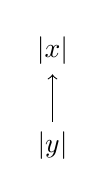
\begin{tikzpicture}[anchor=base, baseline=1.3em, node distance=1.2cm]
\node (y) {\(\lvl{\prc|y|}\)};
\node (x) [above of = y] {\(\lvl{\prc|x|}\)};
\draw[->] (y) -- (x);
\end{tikzpicture}
and
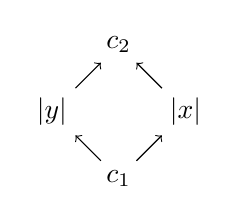
\begin{tikzpicture}[anchor=base, baseline=2.3em, node distance=1.2cm]
\node (c1) {\(c_1\)};
\node (y) [above left of = c1] {\(\lvl{\prc|y|}\)};
\node (x) [above right of = c1] {\(\lvl{\prc|x|}\)};
\node (c2) [above right of = y] {\(c_2\)};
\draw[->] (c1) -- (x);
\draw[->] (c1) -- (y);
\draw[->] (x) -- (c2);
\draw[->] (y) -- (c2);
\end{tikzpicture},
but would be free of violation with \(\lvl{\prc|x|} = \lvl{\prc|y|}\) or
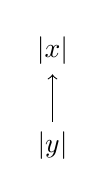
\begin{tikzpicture}[anchor=base, baseline=1.3em, node distance=1.2cm]
\node (y) {\(\lvl{\prc|y|}\)};
\node (x) [above of = y] {\(\lvl{\prc|x|}\)};
\draw[->] (y) -- (x);
\end{tikzpicture}.

\subsubsection{Constructing Security-Flow Matrices}%
\label{subsec:construction}\index{security-flow matrix}

The \ndx{security-flow matrix} of a command is constructed by induction, using
the \ndx{security monoid}. \autoref{subsec:ni-examples} gathers additional
examples with longer discussion.

\paragraph{Base Cases: Assignment and Skip} The security-flow matrix for an
assignment \prc|C|\symbo{p2} simply tracks flows from $\In(\prc|C|)$\symbo{vin}
to $\Out(\prc|C|)$\symbo{vout}:

\begin{definition}[Assignment]%
\label{def:assignment}
Given an assignment \prc|C|\symbo{p2}, we define \(\sfm{\prc|C|}\)\symbo{sfm}
by:
\[
\sfm{\prc|C|}(\prc|x|,\prc|y|)=
%! suppress = EscapeAmpersand
\begin{dcases*}
\vi & if $\prc|x| \in \In(\prc|C|)$,
$\prc|y| \in \Out(\prc|C|)$ and $\prc|x| \neq \prc|y|$ \\
\nv & otherwise
\end{dcases*}
\]\symbo{sfmxy}\symbo{vin}\symbo{vout}\symbo{xvar2}
\end{definition}

\begin{table}
%! suppress = EscapeAmpersand
\begin{tabularx}{\textwidth}{@{}llcX@{}}
\toprule
\prc|C|
& $\Out(\prc|C|)$, $\In(\prc|C|)$\symbo{vin}\symbo{vout}
& $\sfm{\prc|C|}$\symbo{sfm}
& \prc|C| has \ndx{violation}(s) if \ldots \\
\midrule
\prc|w = 3|
& %
$\begin{aligned}
\Out(\prc|C|) &=\{\prc|w|\}    \\
\In(\prc|C|)  &=\emptyset
\end{aligned}$
&
$\begin{pNiceMatrix}[first-row,first-col,baseline=t]
        & \prc|w|\\
\prc|w| &  \nv
\end{pNiceMatrix}$\symbo{nv}
& (Impossible)
\\
\prc|y = x|
& %
$\begin{aligned}
\Out(\prc|C|) &=\{\prc|y|\}    \\
\In(\prc|C|)  &=\{\prc|x|\}
\end{aligned}$
& %
$\begin{pNiceMatrix}[first-row,first-col,baseline=t]
        & \prc|y| & \prc|x|\\
\prc|y| &  \nv\symbo{nv} & \nv \\
\prc|x| &  \vi\symbo{vi} & \nv
\end{pNiceMatrix}$\symbo{nv}\symbo{vi}
& \(\lvl{\prc|y|} < \lvl{\prc|x|}\) or
  \(\lvl{\prc|y|} \orth \lvl{\prc|x|}\).\symbo{secvar}
\\
\prc|w = t[x + 1]|
& %
$\begin{aligned}
\Out(\prc|C|) &=\{\prc|w|\}    \\
\In(\prc|C|)  &=\{\prc|t|, \prc|x|\}
\end{aligned}$
& %
$\begin{pNiceMatrix}[first-row,first-col,baseline=t]
        & \prc|w|   & \prc|t| & \prc|x| \\
\prc|w| & \nv       & \nv     & \nv\\
\prc|t| & \vi       & \nv     & \nv \\
\prc|x| & \vi       & \nv     & \nv
\end{pNiceMatrix}$\symbo{nv}\symbo{vi}
& $\begin{aligned}
\lvl{\prc|w|} &< \lvl{\prc|t|}\text{, }  &
  \lvl{\prc|w|} &\orth \lvl{\prc|t|} \text{,}\\
\lvl{\prc|w|} &< \lvl{\prc|x|}\text{ or\kern-1em} &
  \lvl{\prc|w|} &\orth \lvl{\prc|x|}\text{.}
\end{aligned}$\\
\prc|t[i] = u + j|
& %
$\begin{aligned}
\Out(\prc|C|) &=\{\prc|t|\}          \\
\In(\prc|C|)  &=\{\prc|i|, \prc|u|, \prc|j|\}
\end{aligned}$
& %
$\begin{pNiceMatrix}[first-row,first-col,baseline=t]
        & \prc|t| & \prc|i| & \prc|u| & \prc|j| \\
\prc|t| & \nv     & \nv     & \nv     & \nv \\
\prc|i| & \vi     & \nv     & \nv     & \nv \\
\prc|u| & \vi     & \nv     & \nv     & \nv \\
\prc|j| & \vi     & \nv     & \nv     & \nv
\end{pNiceMatrix}$\symbo{nv}\symbo{vi}
&  $\begin{aligned}
\lvl{\prc|t|} &< \lvl{\prc|i|}\text{,} &
  \lvl{\prc|t|} &\orth \lvl{\prc|i|}\text{,}\\
\lvl{\prc|t|} &< \lvl{\prc|u|}\text{,} &
  \lvl{\prc|t|} &\orth \lvl{\prc|u|}\text{,}\\
\lvl{\prc|t|} &< \lvl{\prc|j|}\text{ or\kern-.6em} &
  \lvl{\prc|t|} &\orth \lvl{\prc|j|}\text{.}
\end{aligned}$ \\
\bottomrule
\caption[Statement examples, sets, and possible violation(s)]
{Statement Examples, Sets, Representations of their Possible Violation(s).}
\label{tab:threecases}
\end{tabularx}
\end{table}

We illustrate in \autoref{tab:threecases} some basic cases: we consider an array
a single entity, and that changing one value in it means being able to access it
completely. More precisely, \prc|t[i]| on the left-hand side of an assignment is
a violation if \(\lvl{\prc|t|} > \lvl{\prc|i|}\) (\resp \(\lvl{\prc|t|} \orth
\lvl{\prc|i|}\))\symbo{secvar}. Indeed, it implies that a lower-class (\resp
orthogonal-class) variable (\prc|i|) can decide where to write in a higher-class
(\resp orthogonal-class) variable (\prc|t|). However, \prc|t[i]| as an
expression (\eg on the right-hand side of an assignment or in a condition, as
discussed in \autoref{sssec:correction}) is acceptable as long as the
variable(s) storing the result of this calculation or dependent on that
condition's truth value have class higher or equal to \prc|t| and \prc|i|
classes.

\begin{definition}[Skip]
We let $\sfm{\prc|skip|}$\symbo{sfm} be the matrix with $0$ rows and columns.
\end{definition}

Identifying $\sfm{\prc|skip|}$\symbo{sfm} with its embeddings, it is the empty
matrix of any size.

\paragraph{Composition as a Commutative Operation}
\label{ni-composition}

The \ndx{security-flow matrix} for a composition of commands is an abstraction
that allows manipulating a sequence of commands as one command with its own
matrix.

%! suppress = EscapeUnderscore
\begin{definition}[Composition]
We let \ensuremath{\sfm{\prc|C$_1$;$\cdots$;C$_n$|}}\symbo{sfm}
be \ensuremath{\sfm{\prc|C$_1$|} + \cdots + \sfm{\prc|C$_n$|}}.
\end{definition}

\newsavebox\compone
\begin{lrbox}{\compone}
\begin{minipage}{.25\linewidth}
\begin{whilelisting}*[numbers=none]
w = w + x;
z = y + 2
\end{whilelisting}
\end{minipage}
\end{lrbox}

\newsavebox\comptwo
\begin{lrbox}{\comptwo}
\begin{minipage}{.25\linewidth}
\begin{whilelisting}*[numbers=none]
x = y * 2;
z = 0
\end{whilelisting}
\end{minipage}
\end{lrbox}

\begin{figure}
\begin{center}
%! suppress = EscapeAmpersand
\begin{tabular}{ccccc}\symbo{nv}\symbo{vi}
\prc|C$_1$| && \prc|C$_2$| && \prc|C$_1$;C$_2$|
\\
$\begin{pNiceMatrix}[first-row,first-col,left-margin=-2pt,right-margin=-2pt]
        & \prc|w|  & \prc|x|  & \prc|y|  & \prc|z| \\
\prc|w| & \nv      & \nv      & \nv      & \nv     \\
\prc|x| & \vi      & \nv      & \nv      & \nv     \\
\prc|y| & \nv      & \nv      & \nv      & \vi     \\
\prc|z| & \nv      & \nv      & \nv      & \nv
\end{pNiceMatrix}$\symbo{nv}\symbo{vi} & + &
$\begin{pNiceMatrix}[first-row,first-col,left-margin=-2pt,right-margin=-2pt]
        & \prc|w|  & \prc|x|  & \prc|y|  & \prc|z| \\
\prc|w| & \nv      & \nv      & \nv      & \nv     \\
\prc|x| & \vi      & \nv      & \nv      & \nv     \\
\prc|y| & \nv      & \vi      & \nv      & \vi     \\
\prc|z| & \nv      & \nv      & \nv      & \nv
\end{pNiceMatrix}$\symbo{nv}\symbo{vi} & = &
$\begin{pNiceMatrix}[first-row,first-col,left-margin=-2pt,right-margin=-2pt]
        & \prc|w|  & \prc|x|  & \prc|y|  & \prc|z| \\
\prc|w| & \nv      & \nv      & \nv      & \nv     \\
\prc|x| & \vi      & \nv      & \nv      & \nv     \\
\prc|y| & \nv      & \vi      & \nv      & \vi     \\
\prc|z| & \nv      & \nv      & \nv      & \nv
\end{pNiceMatrix}$\symbo{nv}\symbo{vi} \\ \\
\usebox\compone && \usebox\comptwo \\
\end{tabular}
\end{center}
\caption[Security-Flow Matrix of compositions]
{Security-Flow Matrix of compositions.}\index{violation}
\label{fig:composition}
\index{security-flow matrix}
\end{figure}

The composition of commands \prc|C$_1$| and \prc|C$_2$|---themselves already the
result of compositions of assignments involving disjoint variables---is
illustrated in~\autoref{fig:composition}. Two important observations:

%! suppress = EscapeUnderscore
\begin{enumerate}
\item
Some existing approaches might consider \prc|C$_1$;C$_2$| as free of
\ndx{violation} even if \(\lvl{\prc|z|} < \lvl{\prc|y|}\), since \(\prc|z = 0|\)
will wipe out the content of \prc|z| and \enquote{cancel} the \ndx{violation}
introduced by \prc|z = y|. The intuition is that an attacker observing the
output (or even all the final values) cannot deduce anything about \prc|z|'s
value (and, transitively\index{information flow!transitive}, about the value of
the higher-class \prc|y|) once the computation is over. Our \enquote{once a
\ndx{violation}, always a violation} approach ignores the fact that
\enquote{ultimately}, this \ndx{violation} may be hidden--the anytime
non-interference\index{non-interference!anytime} guarantee is discussed in
\autoref{subsec:ni-soundness}.
\item
Interestingly, \ensuremath{\sfm{\prc|C$_1$;C$_2$|} =
\sfm{\prc|C$_2$;C$_1$|}}\symbo{sfm} since composition is interpreted as a sum of
matrices over our \emph{commutative} \ndx{security monoid}. While previous
flow-based approaches~\cite{aubert20222,aubert20232,jones2009} require a
\ndx{semi-ring} because composition was handled \emph{via} product of matrices,
the current set-up simplifies the machinery precisely to keep track of past
\ndx{violation}s.
\end{enumerate}

\paragraph{A Correction for Implicit Flows}%
\label{sssec:correction}

To account for implicit flows\index{information flow!implicit}, branchings and
loops require a \emph{correction}. The main idea is that interpreting \prc|if e
then C$_1\;$ else C$_2$| (\resp \prc|while e do C|) require to record that all
the variables modified in \prc|C$_1$| and \prc|C$_2$| (\resp in \prc|C|) depend
on the variables \emph{occurring} in \(\prc|e|\) (as opposed to the assignment
considering the variables \emph{used} by \prc|C|)\symbo{p2}.

%! suppress = EscapeAmpersand
\begin{definition}[Correction]%
\label{def:correction}
The \emph{correction $\corr{\prc|e|}_{\prc|C|}$\symbo{corr} of an expression
\prc|e| on a program \prc|C|} is
\[
\corr{\prc|e|}_{\prc|C|}(\prc|x|,\prc|y|)=
\begin{dcases*}
\vi & if $\prc|x| \in \Occ(\prc|e|)$, $\prc|y| \in \Out(\prc|C|)$ and \(\prc|x|
\neq \prc|y|\) \\
\nv & otherwise
\end{dcases*}
\]\symbo{vout}\symbo{occ}
\end{definition}

Intuitively, the correction states that if the variable \prc|y| is modified in
the body of either branch of the branching or in the body of the loop and
\(\prc|x|\)\symbo{xvar2} occurs in the expression, then there is a violation if
\(\lvl{\prc|y|} < \lvl{\prc|x|}\) or \(\lvl{\prc|y|} \orth
\lvl{\prc|x|}\).\symbo{secvar}

As an example, let us use \autoref{fig:composition} to construct
\ensuremath{\corr{\prc|w x|}_{\prc|C$_1$;C$_2$|}}\symbo{corr}\symbo{p2}, \eg
\prc|w > x|'s correction for \prc|C$_1$;C$_2$|\symbo{p2}. Variables \prc|w| and
\prc|x|\symbo{xvar2}, through the expression \prc|w > x|, control the values of
\prc|w|, \prc|x| and \prc|z| since \prc|C$_1$| and \prc|C$_2$| set those values,
and their execution depend on it, giving:

\[%! suppress = EscapeAmpersand
\begin{pNiceMatrix}[first-row,first-col]
        & \prc|w| & \prc|x| & \prc|y| & \prc|z|\\
\prc|w| & \nv     & \vi     & \nv     & \vi \\
\prc|x| & \vi     & \nv     & \nv     & \vi \\
\prc|y| & \nv     & \nv     & \nv     & \nv \\
\prc|z| & \nv     & \nv     & \nv     & \nv
\end{pNiceMatrix}.\]\symbo{nv}\symbo{vi}\index{violation}

Observe also that in \(\corr{\prc|t[i] != x|}_{\prc|C|}\)\symbo{corr} the
variables \prc|t|, \prc|i| and \prc|x| would be marked as controlling the
variables occurring in \(\Out(\prc|C|)\)\symbo{vout}. However, no constraint
would be imposed between the classes of \prc|t|, \prc|i| and
\prc|x|,\symbo{xvar2} since they would all be required to flow into classes that
are higher or equal to theirs.

\paragraph{Conditionals and Loops}
Following our previous observation, branchings and loops are interpreted
similarly.

%! suppress = EscapeUnderscore
\begin{definition}[Branching]%
\label{def:if}
We let \ensuremath{\sfm{\prc|if e then C$_1\;$ else C$_2$|}} be
\ensuremath{\sfm{\prc|C$_1$;C$_2$|} +
\corr{\prc|e|}_{\prc|C$_1$;C$_2$|}}\symbo{sfm}\symbo{corr}.
\end{definition}

\newsavebox%! suppress = NonMatchingIf
\ifconectwo
\begin{lrbox}{\ifconectwo}
\begin{minipage}{4cm}
%! suppress = FileNotFound
\lstinputlisting[
  mathescape,nolol,frame=none,numbers=none,label={lst:if-else-whl},
  aboveskip=0em,belowskip=0em]{if-else.while}
\end{minipage}
\end{lrbox}

\noindent
Adding \ensuremath{\corr{\prc|w > x|}_{\prc|C$_1$;C$_2$|}}\symbo{corr} to
\ensuremath{\sfm{\prc|C$_1$|} + \sfm{\prc|C$_2$|}}\symbo{sfm} from
\autoref{fig:composition}, we obtain:
\[\mathbb{M} \left(~ \usebox\ifconectwo
\right) \ = \
%! suppress = EscapeAmpersand
\begin{pNiceMatrix}[first-row,first-col]
        & \prc|w| & \prc|x| & \prc|y| & \prc|z|\\
\prc|w| & \nv     & \vi     & \nv     & \vi  \\
\prc|x| & \vi     & \nv     & \nv     & \vi \\
\prc|y| & \nv     & \vi     & \nv     & \vi \\
\prc|z| & \nv     & \nv     & \nv     & \nv
\end{pNiceMatrix}\symbo{vi}\symbo{nv}\text{.}\]

Observe that there is a \ndx{violation} if \(\lvl{\prc|w|} <
\lvl{\prc|x|}\)\symbo{secvar} or \(\lvl{\prc|w|} \orth \lvl{\prc|x|}\) from the
statement $\prc|w = w + x|$, and that there is a \ndx{violation} if
\(\lvl{\prc|x|} < \lvl{\prc|w|}\)\symbo{secvar} or \(\lvl{\prc|x|} \orth
\lvl{\prc|w|}\). The latter comes from the fact that the value of \(\prc|w|\)
will decide if \(\prc|x = y * 2|\) will execute through the expression. To be
free of violations, such a program must be given a class assignment satisfying
\(\lvl{\prc|w|} = \lvl{\prc|x|}\)\symbo{secvar} and the other constraints
recorded in the matrix.

\begin{definition}[Loop]
We let \(\sfm{\prc|while e do C|}\) be \(\sfm{\prc|C|} +
\corr{\prc|e|}_{\prc|C|}\).\symbo{sfm}\symbo{corr}
\end{definition}

\newsavebox\whilec
\begin{lrbox}{\whilec}
\begin{minipage}{4cm}
%! suppress = FileNotFound
\lstinputlisting[
  mathescape,nolol,frame=none,label={array-whl},
  numbers=none,aboveskip=0em,belowskip=0em]{arrays.while}
\end{minipage}
\end{lrbox}
\[\mathbb{M} \left(~ \usebox\whilec
\right) \ = \
%! suppress = EscapeAmpersand
\begin{pNiceMatrix}[first-row,first-col]
& \prc|t| & \prc|i| & \prc|j| & \prc|s1| & \prc|s2| \\
\prc|t| & \nv & \vi & \nv & \vi & \vi \\
\prc|i| & \nv & \nv & \nv & \vi & \vi \\
\prc|j| & \nv & \vi & \nv & \vi & \vi\\
\prc|s1| & \nv & \nv & \nv & \nv & \nv \\
\prc|s2| & \nv & \nv & \nv & \nv & \nv
\end{pNiceMatrix} \]\symbo{nv}\symbo{vi}

Since \prc|s1| and \prc|s2| do not control any other variable, their rows are
all $\nv$s.\symbo{nv} On the other hand, \prc|t|, \prc|i| and
\prc|j|\symbo{xvar2} control the values of \prc|s1|, \prc|s2| and \prc|i|, since
they determine how many times the body will execute.

\subsection{Capturing Anytime Non-Interference}
\label{subsec:ni-soundness}
\index{non-interference!anytime}

In the seminal work of Volpano et al.~\cite[pg.~173]{volpano1996},
\enquote{\textins{s}oundness\index{soundness} \textins{wa}s formulated as a kind
of noninterference property. \textins{\dots I}f a variable $v$ has security
\textins{class $c$}\symbo{seccls}, then one can change the initial values of any
variables whose security levels are not dominated by
\textins{$c$}\symbo{seccls}, execute the program, and the \emph{final value} of
$v$ will be the same, \emph{provided the program terminates successfully}.} (our
emphasis). \emph{Anytime non-interference}\index{non-interference!anytime},
defined below and captured by \lname, inspects the values \emph{while the
program is being executed}. It allows us to
\begin{enumerate*}
\item avoid making assumptions of program \ndx{termination}, or avoid waiting for
termination, and
\item model attackers\index{attacker (adversary)} who are capable of observing
updates to variables at class $c$\symbo{seccls} or lower.
\end{enumerate*}

First, we need to define a notion of \emph{timed} execution, which captures the
idea that an external observer can see updates on variables below a particular
\ndx{security class} in \enquote{real time}.

\begin{definition}[Timed command execution]
Given
\begin{enumerate}
\item a program \prc|C|\symbo{p2} with variables \(\prc|x|_1, \hdots,
\prc|x|_n\)\symbo{xvar2},
\item a class assignment \(\ell : \Occ(\prc|C|) \to
\SC\)\symbo{secasgn}\symbo{seclat},
\item a security class\index{security class} \(\scl{c} \in \SC\)\symbo{seccls},
\item a \emph{time (counter)} \(t \in \mathbb{N}\)\symbo{nat}\symbo{time},
\item and a value list \(\vec{v} = v_1, \hdots, v_n\)\symbo{vecv},
\end{enumerate}
we write
\begin{itemize}

\item \(\prc|C|[\vec{v}]_0\)\symbo{vecv}\symbo{cvec} for the program
\prc|C|\symbo{p2} where the variable \ensuremath{\prc|x$_i$|}\symbo{xvar2} was
assigned \(v_i\)\footnote{Since arrays have a fixed size, we assume, for
simplicity, that a variable \prc|x$_i$| representing an array of size $s$ is
given a value $v_i = v_i^1, \hdots, v_i^s$.}, for \(1 \leqslant i \leqslant n\),

\item  \(\prc|C|[\vec{v} \rightarrow \vec{v'}]_t\)\symbo{cvtm} if, while
executing the commands in \(\prc|C|[\vec{v}]_0\), \ensuremath{\prc|x$_i$|}
contains the value \(v_i'\), for \(1 \leqslant i \leqslant n\) after variables
at class \(\scl{c}\) or lower have been updated \(t\) times.

\end{itemize}
If, after \(t\)\symbo{time} updates, variables at level
\(\scl{c}\)\symbo{seccls} or lower stop being updated, then we let, for all \(t'
> t\)\symbo{time}, \(\prc|C|[\vec{v} \rightarrow \vec{v'}]_t = \prc|C|[\vec{v}
\rightarrow \vec{v'}]_{t'}\)\symbo{cvtm}.
\end{definition}

Deciding whether variables will be updated after \(t\)\symbo{time} may be
difficult in all generality, but simple checks as \eg testing for membership in
\(\Out(\prc|C|')\)\symbo{occ}\symbo{psub} for \(\prc|C|' \subseteq
\prc|C|\)\symbo{p2} the subprogram of \prc|C| that remains to be executed can
give in some cases a rapid answer.

We give below a program along with a class assignment (where the \ndx{security
class} \(\scl{c}\)\symbo{seccls} is grayed out) and two tables containing the
value held by memory locations at time counter \(t\)\symbo{time}. The initial
value lists are \(\vec{v_1} = \prc|1|, \prc|2|, \prc|3|, \prc|4|\)\symbo{vecv}
and \(\vec{v_2} = \prc|5|, \prc|2|, \prc|3|, \prc|4|\). Observe that
\(t\)\symbo{time} is incremented only when values held by variables at or below
\(\scl{c}\)\symbo{seccls} (with the grayed out background) are updated.

\newsavebox\ifconectwoo
%! suppress = NonMatchingIf
\begin{lrbox}{\ifconectwoo}
\begin{minipage}{5cm}
\begin{whilelisting}*[numbers=none]
if (w > x) then
  w = w + x;
  z = y + 2
else
  x = y * 2;
  z = 0
\end{whilelisting}
\end{minipage}
\end{lrbox}

\noindent%
\begin{tabularx}{\textwidth}{@{}l@{\hspace{2em}}l@{}}
\usebox\ifconectwoo &
\begin{tikzpicture}[baseline = 30pt, anchor=base, node distance=1cm]
\node (x) {\(\lvl{\prc|x|}\)};
\node (w) [above left  = .45cm and .08cm of x] {\(\lvl{\prc|w|}\)};
\node (y) [above right = .45cm and .08cm of x] {\(\lvl{\prc|y|}\)};
\node (z) [above right = .45cm and .08cm of w] {\(\lvl{\prc|z|}\)};
\draw[->] (x) -- (w);
\draw[->] (x) -- (y);
\draw[->] (w) -- (z);
\draw[->] (y) -- (z);
\begin{scope}[on background layer]
\node [
  fill=fillcolor, fit=(y), rounded corners=.3cm,
  inner sep=1pt, draw=fillborder] {};
\end{scope}
\end{tikzpicture}\symbo{secvar}
\\ \\
\begin{tabular}{c || c >{
  \columncolor{fillcolor}}c >{\columncolor{fillcolor}}c c }
$t$ & \prc|w| & \prc|x| & \prc|y| & \prc|z| \\ \hline \hline
$0$ & \prc|1| & \prc|2| & \prc|3| & \prc|4| \\ \hline
$1$ & \prc|1| & \prc|6| & \prc|3| & \prc|4| \\
$1$ & \prc|1| & \prc|6| & \prc|3| & \prc|0|
\end{tabular}\symbo{xvar2}
&
\begin{tabular}{c || c >{
  \columncolor{fillcolor}}c >{\columncolor{fillcolor}}c c }
$t$ & \prc|w| & \prc|x| & \prc|y| & \prc|z| \\ \hline \hline
$0$ & \prc|5| & \prc|2| & \prc|3| & \prc|4| \\ \hline
$0$ & \prc|7| & \prc|2| & \prc|3| & \prc|4| \\
$0$ & \prc|7| & \prc|2| & \prc|3| & \prc|5|
\end{tabular}\symbo{xvar2}
\end{tabularx}

\noindent Hence we have \(\prc|C|[\vec{v_1} \rightarrow
\vec{v_1'}]_1\)\symbo{cvtm} and \(\prc|C|[\vec{v_2} \rightarrow \vec{v_2'}]_0 =
\prc|C|[\vec{v_2} \rightarrow \vec{v_2'}]_1\) for \(\vec{v_1'} = \prc|1|,
\prc|6|, \prc|3|, \prc|0|\)\symbo{vecv} and \(\vec{v_2'} = \prc|7|, \prc|2|,
\prc|3|, \prc|5|\).

\begin{definition}[Up-to \(\scl{c}\) equivalence] Given \prc|C|\symbo{p2}, a
class assignment \(\ell : \Occ(\prc|C|) \to
\SC\)\symbo{seccls}\symbo{occ}\symbo{seclat} and \(\scl{c} \in
\SC\)\symbo{seccls}, two values lists \(\vec{v}\)\symbo{vecv} and \(\vec{w}\)
are \emph{up-to \(\scl{c}\) equivalent}, written \(\vec{v} \upce{\scl{c}}
\vec{w}\)\symbo{upce} if \ensuremath{\ell(\prc|x$_i$|) \leqslant \scl{c}
\implies v_i=w_i}\symbo{secvar}. \end{definition}

Intuitively, two value lists are up-to \(\scl{c}\)\symbo{seccls} equivalent if
they agree on the values of the variables of class \(\scl{c}\) or lower:
re-using the example above, we have \(\vec{v_1} \upce{\lvl{\prc|y|}}
\vec{v_2}\)\symbo{upce} but  \(\vec{v_1} \nupce{\lvl{\prc|w|}}
\vec{v_2}\)\symbo{vecv}\symbo{nupce}.

We can now formally state the anytime
non-interference\index{non-interference!anytime} property:

\begin{definition}[Anytime non-interference]%
\label{def:com-ni}
A program \prc|C|\symbo{p2} is \emph{anytime non-interfering for \(\ell :
\Occ(\prc|C|) \to \SC\)}\symbo{occ}\symbo{secasgn}\symbo{seclat} if for all
\ndx{security class} \(\scl{c} \in \SC\)\symbo{seccls}, for all time \(t \in
\mathbb{N}\)\symbo{nat}\symbo{time} and all \(\vec{v}\)\symbo{vecv} and
\(\vec{w}\),
\[
\vec{v}\upce{\scl{c}} \vec{w}, \prc|C|[\vec{v} \rightarrow \vec{v'}]_t,
\prc|C|[\vec{w} \rightarrow \vec{w'}]_t \implies \vec{v'}\upce{\scl{c}}
\vec{w'}\text{.}
\]\symbo{upce}\symbo{cvtm}\symbo{p2}\symbo{vecv}
\end{definition}

Note that we can conclude that the program above is \emph{not} anytime
non-interfering\index{non-interference!anytime} for the given class assignment,
since \(\vec{v_1} \upce{\lvl{\prc|y|}} \vec{v_2}\)\symbo{upce}\symbo{secvar} but
\(\vec{v_1'} \nupce{\lvl{\prc|y|}} \vec{v_2'}\)\symbo{nupce}: we had already
noted, using \lname, that \(\ell(\prc|w|) = \ell(\prc|x|)\)\symbo{secvar} was
required for this program to be anytime
non-interfering\index{non-interference!anytime}. Indeed, this property has a
natural equivalent in \lname, and can be established using it:

\begin{definition}[Non-interfering class assignment]%
\label{def:level-ni}
Given $\sfm{\prc|C|}$\symbo{sfm}, a class assignment \(\ell\)\symbo{secasgn} is
\emph{anytime non-interfering\index{non-interference!anytime} for
\prc|C|\symbo{p2}} iff \prc|C| has no \ndx{violation} (\autoref{def:violation}).
\end{definition}

Note that the trivial class assignment \(\scl{i}\) that assigns to all values
the same \ndx{security class} \(c_i\)\symbo{seccls} is always
non-interfering\index{non-interference}, since in that case \(\scl{i}(\prc|y|) <
\scl{i}(\prc|x|)\) and \(\scl{i}(\prc|y|) \orth \scl{i}(\prc|x|)\) are always
false. Conversely, any program is anytime
non-interfering\index{non-interference!anytime} for \(\scl{i}\), since value
lists are up-to \(c_i\)\symbo{seccls} equivalent if and only if they are equal.

\begin{restatable}[Correspondance]{theorem}{corrthm}\label{thm:corr}
A program \prc|C|\symbo{p2} is anytime
non-interfering\index{non-interference!anytime} for \(\ell\)\symbo{secasgn}
(\autoref{def:com-ni}) if and only if \(\ell\) is anytime non-interfering for
\prc|C| (\autoref{def:level-ni}).
\end{restatable}

The proof is detailed in \autoref{app:proof}, it leverages the idea that only
assignments and corrections can introduce \(\vi\)\symbo{vi} in security-flow
matrices. This mirror the idea that only assignments, loops and branchings can
trigger the update of an element in a value list, hence connecting the two
definitions of anytime non-interference\index{non-interference!anytime}. An
important assumption is that expressions are falsifiable, \eg that if
\ensuremath{\prc|x$_i$| \in \Occ(\prc|e|)}\symbo{occ}\symbo{xvar2}, then there
exists at least one value for \ensuremath{\prc|v$_i$|} that will make \prc|e|
evaluate to \prc|false|, and at least one value that will make it evaluate to
\prc|true|.

\subsection{Interpreting Function Calls in an Anytime Non-Interfering Context}
\label{sec:fct-calls}

We detail below how function calls can be integrated into our analysis. The main
challenge is to nail down the correct interpretation of anytime
non-interference\index{non-interference!anytime} for functions that may have
\ndx{side effect}s or, conversely, that may return a value with a lower class
than its inputs. We start, as a warm-up, by discussing how to add to \lname pure
functions, then functions with \ndx{side effect}s, before finally discussing the
meaning of anytime non-interference\index{non-interference!anytime} for
functions.

\subsubsection{Warm-Up: Pure Functions}%
\label{ssec:pure-fct}

First, let us discuss how \emph{pure} functions can be integrated into \lname.
The first steps are to add \(\emph{fun}(\emph{exp}, \hdots,
\emph{exp})\)\symbo{f} to the expressions, let \prc|f| and \prc|g| range over
function, and to let \ensuremath{\Occ(\prc|f(e$_1$, $\hdots$,e$_n$)|)  =
\prc|f$_{\vec{\mathtt{e}}}$|} for \prc|f$_{\vec{\mathtt{e}}}$| a freshly
introduced variable unique to \prc|f|, \prc|e$_1$|, $\hdots$,
\prc|e$_n$|\symbo{fe}\footnote{This point is clarified at the end of this
subsection.}. Let us illustrate those first steps by interpreting two programs
involving function calls. Simply using the definition of
\ensuremath{\Occ(\prc|f(e$_1$, $\hdots$,e$_n$)|)}\symbo{occ}, and without
changing Definitions~\ref{def:assignment} or~\ref{def:if}, we have:

\newsavebox\purefg
\begin{lrbox}{\purefg}
\begin{minipage}{4cm}
\begin{lstlisting}[
  frame=none,numbers=none,aboveskip=0em,
  belowskip=0em,label={lst:if-else-pure}]
if (g(x, y) > x)
  then y = z
else skip
\end{lstlisting}
\end{minipage}
\end{lrbox}

\begin{table}[h!]
\begin{center}
%! suppress = EscapeAmpersand
\begin{tabular}{@{}llc@{}}
\toprule
\prc|C|\symbo{p2}
& $\Out(\prc|C|)$\symbo{vout}, $\In(\prc|C|)$\symbo{vin}
& $\sfm{\prc|C|}$\symbo{sfm} \\
\midrule
  \prc|x = f(y)|
&
\ensuremath{\begin{aligned}
  \Out(\prc|C|) &=\{\prc|x|\} \\
  \In(\prc|C|)  &=\{\prc|f$_{\mathtt{y}}$|\}
  \end{aligned}}
&
\ensuremath{
\begin{pNiceMatrix}[first-row,first-col,baseline=c]
          & \prc|x| & \prc|y| & \prc|f$_{\mathtt{y}}$| \\
  \prc|x| & \nv     & \nv & \nv \\
  \prc|y| & \nv     & \nv & \nv  \\
  \prc|f$_{\mathtt{y}}$|  & \vi & \nv & \nv
  \end{pNiceMatrix}}\symbo{nv}\symbo{vi}\symbo{fe}
\\
  \usebox\purefg
&
\ensuremath{\begin{aligned}
  \Out(\prc|C|) &=\{\prc|y|\}  \\
  \In(\prc|C|)  &=\{\prc|g$_{\mathtt{x}, \mathtt{y}}$|, \prc|x|, \prc|z|\}
  \end{aligned}}
&
\ensuremath{
\begin{pNiceMatrix}[first-row,first-col,baseline=c]
        & \prc|x| & \prc|y| & \prc|z| & \prc|g$_{\mathtt{x}, \mathtt{y}}$| \\
\prc|x| &  \nv    & \vi     & \nv     & \nv \\
\prc|y| & \nv     & \nv     & \nv     & \nv \\
\prc|z| & \nv     & \vi     & \nv     & \nv \\
\prc|g$_{\mathtt{x}, \mathtt{y}}$| & \nv & \vi & \nv & \nv
\end{pNiceMatrix}\symbo{nv}\symbo{vi}}
\\
\bottomrule
\end{tabular}
\end{center}
\caption[Anytime non-interference with pure functions]
{Anytime non-interference with pure functions.}
\label{tab:func}\index{non-interference!anytime}
\end{table}

It may seem surprising that \prc|y|\symbo{xvar2} does not occur in the
\(\In(\prc|C|)\)\symbo{vin} sets, considering that its value may affect the
output of the function call, hence controlling indirectly the out-variables.
This design choice \emph{lets the class assignment handle this decision}. The
core idea is that the level assignment \(\ell : \Occ(\prc|C|) \to
\SC\)\symbo{secasgn}\symbo{occ}\symbo{seclat} now additionally needs to assign a
class (or a collection of constraints) to each
\prc|f$_{\vec{\mathtt{e}}}$|\symbo{fe} variable. Multiple design choices exist,
\eg

\begin{itemize}
\item \ensuremath{\ell(\prc|f$_{\vec{\mathtt{e}}}$|)}\symbo{secasgn}\symbo{fe}
can be a constant class \(\scl{c}\)\symbo{seccls}, reflecting the fact that all
function outputs should be assigned the same \ndx{security class} regardless of
the classes assigned to its inputs,

\item \ensuremath{\ell(\prc|f$_{\vec{\mathtt{e}}}$|)}\symbo{secasgn}\symbo{fe}
can be a function of \(\lvl{\prc|x|}\)\symbo{secvar} for \(\prc|x| \in
\Occ(\mathtt{e}_1) \cup \cdots \cup \Occ(\mathtt{e}_n)\)\symbo{occ}\symbo{xvar2}
such as the supremum, the infimum (written \(\max\) and \(\min\)), the first
projection \(\pi_1\), etc.

\item \ensuremath{\ell(\prc|f$_{\vec{\mathtt{e}}}$|)}\symbo{secasgn}\symbo{fe}
could otherwise depends on the particular structure of \(\vec{\mathtt{e}}\), \eg
be the supremum if a variable whose class is above a particular threshold
occurs, a constant otherwise, etc.
\end{itemize}

This adds \enquote{external} constraints to our definition of \ndx{violation}:
\emph{in addition} of having to provide a level assignment meeting the condition
of \autoref{def:violation}, one has to check that the constraints given
on the classes of the \prc|f$_{\vec{\mathtt{e}}}$|\symbo{fe} variables are met.
As an additional benefit, this allows to handle functions with \(0\) parameters,
since the flow from the argument(s, or lack thereof) to the function's output
need not to be tracked in the \ndx{security-flow matrix}.

Going back to our first example above, if we consider that \prc|f|'s\symbo{f}
output class must be strictly higher than its input class, then we have the
additional requirement that \ensuremath{\lvl{\prc|f$_{\mathtt{x}}$|} >
\lvl{\prc|x|}}\symbo{secvar}\symbo{xvar2}\symbo{fe} for each variable
\prc|x|\symbo{xvar2} such that \prc|f$_{\mathtt{x}}$|\symbo{fe} occurs in
$\sfm{\prc|C|}$\symbo{sfm}. Hence, our first program \prc|C|\symbo{p2} would be
free of \ndx{violation}s with
\begin{tikzpicture}[anchor=base, baseline=1.3em, node distance=1cm]
\node (y) {\(\lvl{\prc|y|}\)};
\node (fy) [above of = y] {\ensuremath{\lvl{\prc|f$_{\mathtt{y}}$|}}};
\node (x) [above of = fy] {\(\lvl{\prc|x|}\)};
\draw[->] (y) -- (fy);
\draw[->] (fy) -- (x);
\end{tikzpicture}\symbo{secvar}
and
\begin{tikzpicture}[anchor=base, baseline=1.3em, node distance=1cm]
\node (y) {\(\lvl{\prc|y|}\)};
\node (fy) [above of = y]
  {\ensuremath{\lvl{\prc|f$_{\mathtt{y}}$|} = \lvl{\prc|x|}}};
\draw[->] (y) -- (fy);
\end{tikzpicture}
, but it would have a violation with
\begin{tikzpicture}[anchor=base, baseline=2.3em, node distance=1.2cm]
\node (c) {\(c\)};
\node (y) [above left of = c] {\(\lvl{\prc|y|}\)};
\node (fy) [above right of = c]
  {\ensuremath{\lvl{\prc|f$_{\mathtt{y}}$|}}};
\node (x) [above left of = fy] {\(\lvl{x}\)};
\draw[->] (c) -- (y);
\draw[->] (c) -- (fy);
\draw[->] (fy) -- (x);
\draw[->] (y) -- (x);
\end{tikzpicture},
even if this latter class assignment would have met the requirements of
\autoref{def:violation}.

The rest of the interpretation is the same, even $\sfm{\prc|C|}$\symbo{sfm}
remains a $|\Occ(\prc|C|)|\times |\Occ(\prc|C|)|$\symbo{occ} matrix, since
\prc|f$_{\vec{\mathtt{e}}}$|\symbo{fe} variables are defined as occurring in
\prc|C|\symbo{p2}. The only tedious aspect is to handle the introduction of
\prc|f$_{\vec{\mathtt{e}}}$|\symbo{fe} variables elegantly.
One would want \eg
\begin{align*}
\Occ(\prc|f(x + y))|)  &=  \Occ(\prc|f(x - y))|) && \text{ and } &
\Occ(\prc|f(x + 3))|)  &=  \Occ(\prc|f(x - 5))|)
\shortintertext{
  but relying on \emph{the set} \(\Occ(\mathtt{e}_1)
  \cup \cdots \cup \Occ(\mathtt{e}_n)\) would not be correct,
  as one would want \eg}
\Occ(\prc|f(x, y))|) & \neq  \Occ(\prc|f(y, x))|) && \text{ and } &
\Occ(\prc|f(x, x, y))|)  &\neq  \Occ(\prc|f(x, y, y))|)\text{.}
\end{align*}
A more precise definition of function type signature, capable of handling
repetition and swapping in the argument list, would be required but presents no
challenge.

\subsubsection{Completing the Picture: Functions With Side Effects}
\label{ssec:impure-fct}\index{side effect}

Our development so far assumes that the only way a function can \ndx{leak}
information is through its return value. Considering functions with \ndx{side
effect}s (such as \prc|print|, \prc|read|, accessing a non-local variable,
passing argument by reference, etc.) increases expressivity of
\lname,\index{expressiveness} but requires to discuss more precisely what is
meant by anytime non-interfering\index{non-interference!anytime} function calls.

We first focus on how effects can be integrated into \lname. Interestingly, the
column \prc|f$_{\vec{\mathtt{e}}}$|\symbo{fe} always remains empty, since the
variable \prc|f$_{\vec{\mathtt{e}}}$|\symbo{fe} will never be in an
\(\Out\)\symbo{vout} set (it never \enquote{receives} a value). Hence, we can
use its out-variable to store information about its possible \ndx{side effect}s.
To this end, we now \enquote{split} \prc|f$_{\vec{\mathtt{e}}}$|\symbo{fe} into
\prc|f$^{\mathtt{in}}_{\vec{\mathtt{e}}}$|\symbo{fein} (on the row) and
\prc|f$^{\mathtt{out}}_{\vec{\mathtt{e}}}$| (on the column) for each
\enquote{signature} \prc|f(e$_1$, $\hdots$,e$_n$)|. This convention is
illustrated in \autoref{ex:fct} with another example of \emph{pure} functions.

To account for effects, the expression \(\emph{fun}(\)\emph{exp}, \ldots,
\emph{exp}\()\) should now be treated as a \emph{command \emph{and} an
expression}. We then edit the definition of the variables occurring in
\prc|f(e$_1$, $\hdots$,e$_n$)| (henceforth simply denoted
\prc|f($\vec{\mathtt{e}}$)|) and in $\vec{\mathtt{e}}$ to get a more complete
picture:
\begin{align*}
\Occ(\prc|f($\vec{\mathtt{e}}$)|) & = \prc|f$^{\mathtt{in}}_{\vec{\mathtt{e}}}$|
& \Occ(\vec{\mathtt{e}}) & =
\begin{dcases}
\Occ(\mathtt{e}_1) \cup \cdots \cup \Occ(\mathtt{e}_n) & \text{ if } n > 0\\
\prc|f$^{\mathtt{in}}_{\emptyset}$| & \text{ otherwise}\\
\end{dcases}\symbo{fein}
\shortintertext{with the \enquote{otherwise} case above handling
functions with 0 parameters. We then let}
\sfm{\prc|f($\vec{\mathtt{e}}$)|} & = \sfm{\prc|skip|}
\hspace{-1.25em} & \sfmb{\prc|C|} & =
\sum_{\mathclap{\prc|f($\vec{\mathtt{e}}$)| \subseteq \Occ(\prc|C|)}}
\sfm{\prc|f$^{\mathtt{out}}_{\vec{\mathtt{e}}}$ = $\;
\vec{\mathtt{e}}$|} + \sfm{\prc|C|}
\end{align*}\symbo{feout}\symbo{occ}\symbo{sfmb}\symbo{f}
and study \sfmb{\prc|C|}\symbo{sfmb} moving forward, where the above definition
interprets all function calls as assignments and then interpret the rest of the
program as before, skipping the commands calling a function without using their
return value. \autoref{tab:fct-effect} gathers examples of programs involving
effectful functions. The last example follows our definitions, but may be hard
to unpack: the critical point is to see that
\prc|g$^{\mathtt{in}}_{\emptyset}$|\symbo{fein} controlling the values of
\prc|x| and \prc|g$^{\mathtt{out}}_{\emptyset}$|\symbo{feout} reflects the fact
that \prc|g|\symbo{f} \enquote{on its own} (\ie without any input) will decide
of its output and hence if \prc|x = 0| will execute.

\newsavebox\effectif
\begin{lrbox}{\effectif}
\begin{lstlisting}[
  frame=none,numbers=none,aboveskip=0em,
  belowskip=0em,label=effectif]
if (g()==1)
  then x = 0
else skip
\end{lstlisting}
\end{lrbox}

\begin{table}
  %! suppress = EscapeAmpersand
\begin{tabular}{@{}lllc@{}}
\toprule
  \prc|C|\symbo{p2}
  & $\sfmb{\prc|C|} = \cdots$\symbo{sfmb}
  & $\Out(\prc|C|)$, $\In(\prc|C|)$\symbo{vout}\symbo{vin}
  & $\sfmb{\prc|C|}$ \\
\midrule
  \prc|g(x + y)|
  &
  \ensuremath{\begin{aligned}
  & \sfm{\prc|g$^{\mathtt{out}}_{\mathtt{x}, \mathtt{y}}$ = x + y|} \\
  & + \sfm{\prc|skip|}
  \end{aligned}}\symbo{feout}
  &
  \ensuremath{\begin{aligned}
  \Out(\prc|C|) &=\{\prc|g$^{\mathtt{out}}_{\mathtt{x}, \mathtt{y}}$|\} \\
  \In(\prc|C|)  &=\{\prc|x|, \prc|y|\}
  \end{aligned}}
  &
  \ensuremath{
  \begin{pNiceMatrix}[first-row,first-col,baseline=c]
          & \prc|x| & \prc|y| & \prc|g$^{\mathtt{out}}_{\mathtt{x}, \mathtt{y}}$| \\
  \prc|x| & \nv     & \nv     & \vi \\
  \prc|y| & \nv     & \nv     & \vi  \\
  \prc|g$^{\mathtt{in}}_{\mathtt{x}, \mathtt{y}}$| & \nv & \nv & \nv
  \end{pNiceMatrix}\symbo{nv}\symbo{vi}\symbo{fein}}
  \\[1.6em]
  \prc|x = f(y)|
  &
  \ensuremath{\begin{aligned}
  & \sfm{\prc|f$^{\mathtt{out}}_{\mathtt{y}}$ =  y|} \\
  & + \sfm{\prc|x = f(y)|}
  \end{aligned}}
  &
  \ensuremath{\begin{aligned}
  \Out(\prc|C|) &=\{\prc|x|, \prc|f$^{\mathtt{out}}_{\mathtt{y}}$|\} \\
  \In(\prc|C|)  &=\{\prc|y|, \prc|f$^{\mathtt{in}}_{\mathtt{y}}$|\}
  \end{aligned}}
  &
  \ensuremath{
  \begin{pNiceMatrix}[first-row,first-col,baseline=c]
          & \prc|x| & \prc|y| & \prc|f$^{\mathtt{out}}_{\mathtt{y}}$| \\
  \prc|x| & \nv     & \nv     & \nv \\
  \prc|y| & \nv     & \nv     & \vi \\
  \prc|f$^{\mathtt{in}}_{\mathtt{y}}$| & \vi & \nv & \nv
  \end{pNiceMatrix}\symbo{nv}\symbo{vi}}
\\[1.8em]
  \usebox\effectif
  &
  \ensuremath{\begin{aligned}
  & \corr{\prc|g()==1|}_{\prc|x=0;skip|}\\
  & + \sfm{\prc|x = 0|} \\
  & + \sfm{\prc|g$^{\mathtt{out}}_{\mathtt{\emptyset}}$ = |}
    + \sfm{\prc|skip|} \\
  \end{aligned}}
  &
  \ensuremath{\begin{aligned}
  \Out(\prc|C|) &=\{\prc|x|, \prc|g$^{\mathtt{out}}_{\emptyset}$|\} \\
  \In(\prc|C|)  &= \emptyset
  \end{aligned}}
  &
  \ensuremath{
  \begin{pNiceMatrix}[first-row,first-col,baseline=c]
          & \prc|x| & \prc|g$^{\mathtt{out}}_{\emptyset}$| \\
  \prc|x| &  \nv    & \nv\\
  \prc|g$^{\mathtt{in}}_{\emptyset}$| & \vi & \vi
  \end{pNiceMatrix}\symbo{nv}\symbo{vi}}
\\
\bottomrule
\end{tabular}
\caption[Statement examples, interpretation and sets involving effects]
{Statement Examples, Interpretation and Sets -- Involving Effects.}
\label{tab:fct-effect}\index{side effect}
\end{table}

This interpretation entails the following two principles:

\begin{itemize}
\item An effectful\index{side effect} function is completely transparent: the
first example of \autoref{tab:fct-effect} requires
\ensuremath{\ell(\prc|g$^{\mathtt{out}}_{\mathtt{x}, \mathtt{y}}$|) \geqslant
\max (\ell(\mathtt{y}),
\ell(\mathtt{x}))}\symbo{secasgn}\symbo{feout}\symbo{secvar}, \eg as if
\prc|g|\symbo{f} is revealing all the data it is processing.

\item A function can nevertheless have
\ensuremath{\ell(\prc|f$^{\mathtt{in}}_{\vec{\mathtt{e}}}$|)}
\symbo{secasgn}\symbo{fein} be less than or orthogonal to the level of its
arguments. This means that a function can have a return value that is
independent of its arguments, \eg a \prc|success| or \prc|failure| code in
displaying the arguments at the screen.
\end{itemize}

Those principles can be both desirable and are not incompatible.
Indeed, a program

\newsavebox%! suppress = NonMatchingIf
\ifsecret
\begin{lrbox}{\ifsecret}
\begin{minipage}{.4\textwidth}
\begin{whilelisting}*[numbers=none,label=secret]
success = print(secret);
if (success==0)
  then x++
else x--
\end{whilelisting}
\end{minipage}
\end{lrbox}

\noindent\usebox\ifsecret{ }\hfill{}with the class assignment
\hspace{-4em}
\begin{minipage}{.37\textwidth}
\begin{tikzpicture}[anchor=base, baseline=1.3em, node distance=1.2cm]
\node (y) { \ensuremath{\lvl{\prc|success|} =
  \lvl{\prc|print$^{\mathtt{in}}_{\mathtt{secret}}$|}}};
\node (fy) [above of = y] {\(\lvl{\prc|x|}\)};
\node (x) [above of = fy] {\ensuremath{\lvl{\prc|secret|} =
  \lvl{\prc|print$^{\mathtt{out}}_{\mathtt{secret}}$|} }};
\draw[->] (y) -- (fy);
\draw[->] (fy) -- (x);
\end{tikzpicture}\symbo{secvar}\symbo{fein}\symbo{feout}
\end{minipage}

\noindent should be considered as anytime
non-interfering:\index{non-interference!anytime} a user having access to
\prc|secret|'s class can see its value be displayed on the screen, but an
attacker having access to at most \prc|x|'s class cannot infer \prc|secret|'s
value, despite being able to access the return value of
\prc|print(secret)|---which is constantly set to the lowest class available.

Three challenges remain:
\begin{itemize}

\item The intuitive reading of our security-flow matrices\index{security-flow
matrix} is lost. For example, since \(\prc|y| \notin \In(\prc|x = f(y))|)\),
\(\sfmb{\prc|x = f(y)|}(\prc|x|, \prc|y|) \neq
\vi\)\symbo{vi}\symbo{vin}\symbo{sfmb}, and \prc|y|\symbo{xvar2} is not recorded
as impacting the value of \prc|x|\symbo{xvar2}. This design choice is a
\emph{feature}, as it does not \enquote{force} \prc|y| to control \prc|x|'s
value when processed through \prc|f|: this allows finer constraints on the level
of \prc|f$^{\mathtt{in}}_{\mathtt{y}}$|\symbo{fein}.

\item It rigidly assumes that functions with \ndx{side effect}s will reveal all
their data at all times. This conservative approach is also a feature, but could
be tuned by refining how constraints for
\prc|f$^{\mathtt{out}}_{\vec{\mathtt{e}}}$|\symbo{feout} class assignments are
recorded.

\item Developing a definition of anytime
non-interference\index{non-interference!anytime} for programs with \ndx{side
effect}s (\autoref{def:com-ni}) will requires to develop a notion of external
observer and of contextual equivalences, to correctly account for \ndx{side
effect}s and multiple communication channels.

\end{itemize}

We believe that those issues can be addressed by developing a richer theory that
incorporates \emph{external knowledge on functions}, but reserve it for future
work.

\subsection{Practical Applications and Comparison}\label{sec:apps}

\subsubsection{Implementing the Anytime Non-interference Logic}\label{sec:analyzer}
\index{non-interference!anytime}

We have created a prototype static analyzer \tool that implements the \lname
logic. The way matrices are composed in \lname is a key feature in making the
analysis straightforward and efficient in practice. Because composition order is
irrelevant (\autoref{ex:composition-order}), it suffices to represent matrices
as hash maps where composition is a union of maps.

The \tool analyzer accepts as input a program file written in
\texttt{\ndx{Java}}. It first translates the program into a \ndx{parse tree}
(without optimizations), then analyzes the tree based on the rules of \lname.
The analysis is recursive over the methods of a \texttt{\ndx{Java}} class.
Obtaining a sound result requires a \prc|Java| method fully expressible in the
\lname \ndx{grammar} (\autoref{fig:grammar}). Commands that are not covered are
highlighted by \tool and the analyzer outputs a partial result. This handling
assists the continued development of \lname. Currently, it already handles all
the examples from~\autoref{subsec:ni-examples}.

The outlined engineering choices have multiple advantages. \texttt{\ndx{Java}}
is frequently used to implement taint\index{taint analysis} analyzers, an
instance of \ndx{non-interference} fixed to two \ndx{security class}es. \tool is
thus prepared for a similar use case. Since \prc|Java| compiles into
\ndx{bytecode}\index{Java bytecode}, a kind of intermediate stack language, it
enables program analysis at multiple language representations. Although compiler
optimizations could reduce the rate of false alarms, \eg by eliminating
dead-code, it would artificially inflate the analysis \ndx{precision} and thus we
prefer our strategy. Currently, \tool produces security-flow
matrices\index{security-flow amtrix} for input programs. The security flow
matrices serve as basis for the extended applications, including the directions
presented next.

\begin{description}
\item[Preservation of anytime non-interference.]\index{non-interference!anytime}
The \lname logic does not require much language structure; in particular, it
assumes no language-specific syntactic features. It is possible to map its
\ndx{grammar} to numerous language representations, including intermediate
representations\index{intermediate representation} and bytecode\index{bytecode}.
Comparing security-flow matrices\index{security-flow matrix} of the same program
at different representations enables analyzing preservation of security
properties and detecting compilation issues.

\item[Security class inference.]\index{security class inference}
When \ndx{security class}es of variables are known partially, it is possible to
infer them for all variables. The inference requires a \ndx{security-flow
matrix}, an information flow policy\index{information flow!policy}, and the
known class assignments. The inference is then framed as a satisfiability
problem. If a satisfactory assignment exists, it provides the security classes
for all variables. This application is similar to type inference, but requires
no program as input. Further, the same \ndx{security-flow matrix} can be easily
evaluated against different information flow policies\index{information
flow!policy}.

\item[Taint analysis.]\index{taint analysis}
Taint analysis detects information flow issues between a high source and a low
sink. Aside a program, the sources and sinks are necessary, and analyzers
commonly assume them as inputs. The analyzers then compete on \ndx{precision} along
various axes: path-coverage, syntax-coverage, context-sensitivity, false alarm
rate, \etc. Taint analysis can be formulated with security-flow
matrices\index{security-flow matrix} by analyzing source to sink connectivity.
\end{description}

\subsubsection{Circumventing Termination-insensitivity via Distribution}
\label{subsub:termination}

Several real-world programs are non-terminating by design: web servers, embedded
systems, and cyber-physical systems are among the examples. While the programs
can terminate, the \ndx{termination} events are infrequent and uncharacteristic
of standard behavior. Security analyses that can handle absence of termination
are necessary to support such programs.

Anytime non-interference\index{non-interference!anytime} is
\ndx{termination}-insensitive\index{non-interference!termination-insensitive}
and compatible with the study of non-terminating programs. However,
termination-insensitivity is too weak to guard against untrusted code, \eg
execution of the \prc|eval| command. To offer an alleviation strategy, we
present an approach to distribute security-sensitive computation. This way,
computations that require elevated security checks are handled separately from
trusted code.

The idea is to pair \lname with a \emph{distribution
analysis}~\cite{aubert20232} that detects disjoint program fragments. That
program fragments are disjoint means there exists no exchange of variable data
between program fragments. The judgement of disjointness is derived via a sound
\ndx{data flow analysis} that guarantees the property. It is then permissible to
execute the program fragments in separate execution contexts. Although the
distribution analysis naturally fits parallel computations, it is not restricted
to this use case. We conjecture it offers broader utility here, to ensure
program security.

To combine the two analysis, we first analyze a program with \lname to identify
its \ndx{information flow} constraints. Then, we use the distribution analysis
to identify the program's distribution potential. Merging the results, the
disjoint program fragments are assigned appropriate \ndx{security class}es. The
fragments are then allocated to different execution contexts, where each
fragment can have a different \ndx{security class} designation. This way, a
program must not adhere to a monolithic security strategy, but can have a
finer-grained strategy based on its content. Due to paper scope, we reserve a
detailed treatment for an extended version.

\subsubsection{Overview of Alternative and Related Approaches}
\label{sec:ni-related-works}

In \ndx{language-based security}, \ndx{non-interference} is commonly achieved
through \ndx{security type system}s. Type theoretic \ndx{non-interference}
provides strong end-to-end \ndx{confidentiality} guarantees in a static and
scalable way. Initiating from the seminal work of Volpano et
al.~\cite{volpano1996}, \ndx{security type system}s have been extended to
consider \ndx{non-interference} under numerous paradigms, including
concurrency~\cite{volpano1998,derakhshan2024,frumin2021}\index{concurrent
programs}, formal reasoning~\cite{nelson2020,frumin2021}, \ndx{secure
compilation}~\cite{barthe2004}, \etc. A major challenge among the \ndx{security
type system}s is \emph{\ndx{declassification}}, a kind of security
\ndx{downgrading} operation~\cite{cecchetti2017}. A \emph{downgrading}
mechanisms permits elevating the security judgement around control-flow
constructs then lowering it afterward. In other words, information is allowed to
flow contrary to the policy~\cite{cecchetti2017}. The mechanism is necessary to
increase the expressive power\index{expressiveness} of \ndx{security type
system}s. However, \ndx{downgrading} is generally not safe~\cite{derakhshan2024}
and eliminates the strong compositional\index{compositionality} guarantees of
\ndx{non-interference}~\cite{cecchetti2017}. In practice, \ndx{security type
system}s are challenging to use because they modify the programming language. A
program must be annotated with security types and compiled with non-standard
tools that can enforce the types~\cite{lamba2024}. There is also a stark
contrast in \ndx{expressiveness} of theoretical and practical systems.
\Eg~\cite{huang2014} categorically excludes implicit flows\index{information
flow!implicit}.

The \ndx{Dependency Core Calculus} (DCC)~\cite{abadi1999b} is conceptually
related to \lname. The DCC is an extension of
lambda-calculus\index{\(\lambda\)-calculus}, framed around the notion of
\ndx{data dependence}, of which \ndx{non-interference} is an instance. Though
similarly rooted in dependency analysis\index{dependence analysis} \lname
originates from works of implicit computational complexity (ICC). It is a
refinement of~\cite{moyen20172,aubert20232}, but \lname required significant
adjustment, particularly around matrix composition and functions.

Implicit computational complexity studies machine-free characterizations of
\ndx{complexity class}es by introducing \emph{restrictions} in programming
languages that in turn guarantee semantic properties~\cite{dallago2011}. A
critical idea is that ICC techniques can benefit from, and offer support in,
other analytic domains. The use of ICC techniques is such extended ways is an
emerging research topic. Previously, a \ndx{non-interference} \ndx{type
system}\index{security type system} provided a foundation for a series of
complexity-theoretic results~\cite{marion2011,hainry2023}. In the opposite
direction, an ICC system was applied to cryptographic\index{cryptography}
proofs~\cite{baillot2019}. Although \lname has transformed from its origins to
not enforce complexity bounds, it reinforces the bidirectional connection
between ICC and \ndx{language-based security}.

\subsection{Conclusion: Strengths, Limitations and Future Directions}
\label{sec:conclusion}

Anytime non-interference\index{non-interference!anytime} detects violations at
any program point, enforcing a finer-grained security policy\index{information
flow!policy} than classic non-interference\index{non-interference} that is
defined in terms of inputs and outputs. We have presented \lname, a sound and
compositional program logic, that captures the semantic security property of
anytime non-interference\index{non-interference!anytime} in \ndx{imperative
programs}. The logic assigns security flow matrices\index{security-flow matrix}
to commands where the matrices represent the program's potentially interfering
\ndx{information flow}s. The logic is lightweight and does not require program
annotations, specialty compilers, and adds no run-time overhead. Beside the
compelling theory, \lname can be implemented to obtain automated security
analysis in practice. We have constructed a prototype static analyzer \tool to
analyze \texttt{\ndx{Java}} programs. By extension, \tool can support a range of
applications, \eg \ndx{security class inference}, \ndx{taint analysis}, and
security preservation analysis.

Although the utility of \lname is encouraging, the development is still mainly
theoretical. Our immediate priority is enriching the syntax with effectful
functions and object oriented constructs. For additional strength, we hope to
mechanize the theory. On the practical side, the prototype analyzer has room for
enhancements. It already computes security-flow matrices\index{security-flow
matrix}, but an extension to the applications requires additional engineering
steps. With the current syntax coverage, experimental comparisons are still out
of scope. In the meantime, \lname provides an promising avenue for security
analysis and future enhancements.

\clearpage

\subsection{Appendix A: Proof of \autoref{thm:corr}}\label{app:proof}

A first useful observation is that if \(\prc|C|' \subseteq
\prc|C|\)\symbo{psub}\symbo{p2}, then \(\sfm{\prc|C|'}\)\symbo{sfm} is included
in \(\sfm{\prc|C|}\)\symbo{sfm}, in the sense that \(\sfm{\prc|C|'}(\prc|x|,
\prc|y|) = \vi \implies \sfm{\prc|C|}(\prc|x|, \prc|y|) =
\vi\)\symbo{sfmxy}\symbo{vi}. This simple observation comes from our
\enquote{additive} interpretation of commands, and is useful in proving our
theorem. One should also note that if \(\ell\)\symbo{secasgn} is not anytime
non-interfering for \prc|C|'\symbo{psub}, then any class assignment extending
\(\ell\)\symbo{secasgn} to \(\Occ(\prc|C|)\)\symbo{occ} is not anytime
non-interfering for \prc|C|\symbo{p2}.\index{non-interference!anytime}

\corrthm*

\begin{proof}
Let us assume given \prc|C|, \(\ell : \Occ(\prc|C|) \to
\SC\)\symbo{occ}\symbo{seclat}, and that $\sfm{\prc|C|}$\symbo{sfm} has been
computed.

\begin{description}
\item[For the if part]

Suppose that \(\ell\)\symbo{secasgn} is anytime
non-interfering\index{non-interference!anytime} for \prc|C|\symbo{p2}, but that
\prc|C| is not anytime non-interfering for \(\ell\)\symbo{secasgn} . Then there
must exist a class \(\scl{c} \in \SC\)\symbo{seccls}\symbo{seclat} and a counter
\(t\) such that for some \(\vec{v}\)\symbo{vecv} and \(\vec{w'}\),
\begin{multicols}{2}
\noindent%
\begin{align}
\vec{v}\symbo{vecv} & \upce{\scl{c}}\symbo{upce} \vec{w} \label{eq:equi-level}\\
\prc|C|[\vec{v} &\rightarrow \vec{v'}]_t\symbo{cvtm}
\end{align}%
\begin{align}
\prc|C|[\vec{w} &\rightarrow \vec{w'}]_t\symbo{cvtm} \\
\vec{v'} &\nupce{\scl{c}}\symbo{nupce} \vec{w'}
\end{align}
\end{multicols}

For \(\nupce{\scl{c}}\)\symbo{nupce} the negation of
\(\upce{\scl{c}}\)\symbo{upce}, \ie there must exists
\ensuremath{\prc|x$_i$|}\symbo{xvar2} such that
\begin{multicols}{2}
\noindent
\begin{align}
\ell(\prc|x$_i$|) \leqslant \scl{c} \label{eq:xi-level}
\end{align}
\begin{align}
v_i' \neq w_i' \label{eq:re-assign}
\end{align}\symbo{vecv}\symbo{secvar}
\end{multicols}
For \autoref{eq:re-assign} to hold, it must be the case that \prc|C|\symbo{p2}
contains a statement of the form \prc|x$_i$ = e$_1$|\footnote{Which can be
\prc|t[e$_1^1$]= e$_1^2$|, in which case we let  \ensuremath{\Occ(\prc|e$_1$|) =
\Occ(\prc|e$_1^1$|) \cup \Occ(\prc|e$_1^2$|)}\symbo{occ} and carry out the same
reasoning.}, possibly guarded by \prc|while| and \prc|if| statements using the
expressions  \ensuremath{\prc|e$_2$|, \hdots, \prc|e$_n$|}. Let
\ensuremath{\prc|x$_1$|, \hdots, \prc|x$_m$| = \bigcup_{j=1}^n
\Occ(\prc|e$_j$|)}\symbo{occ}, and observe that since by
\autoref{eq:equi-level} our input value lists are up-to
\(\scl{c}\)\symbo{seccls} equivalent, it must be the case that there exists \(j
\in \{1, \hdots, m\}\) such that
\begin{align}
\ell(\prc|x$_j$|) > \scl{c} \text{ or } \ell(\prc|x$_j$|) \orth \scl{c} \text{,}
\label{eq:xj-level} \end{align}otherwise \autoref{eq:re-assign} could not
hold\footnote{To be more rigorous, it could be the case that the classes of
\ensuremath{\prc|x$_1$|, \hdots, \prc|x$_m$|} are $\scl{c}$ or below, but that
\emph{one of them is itself} impacted by a variable at a higher or incomparable
class. To handle, this case, one simply replaces \prc|x$_i$| and \prc|x$_j$|
with those \enquote{problematic} variables, decreases the counter \(t\) to when
the value of the one with the lower class was changed, and carry out the same
reasoning, possibly repeating this step again. Since \(t\) decreased, we are
guaranteed to identify \enquote{the first} anytime
non-interference\index{non-interference!anytime} \ndx{violation} and to reason
about it.}. Furthermore, thanks to \autoref{eq:xi-level} we know that
\begin{align}
j \neq i\text{.} \label{eq:i-not-j}
\end{align}

Let \(\prc|C|'\)\symbo{psub} be the smallest sub-program of
\(\prc|C|\)\symbo{p2} where \prc|x$_i$ = e$_1$| occurs and either
\ensuremath{\prc|x$_j$| \in \Occ(\prc|e$_1$|)}\symbo{occ} or \prc|x$_j$| occurs
in the condition of a \prc|while| or \prc|if| command guarding the command
\prc|x$_i$ = e$_1$|. Intuitively, \(\prc|C|'\)\symbo{psub} has one of the
following forms:
\vspace{.25em}

\begin{minipage}[t]{.3\linewidth}
\begin{whilelisting}*[mathescape,numbers=none]
x$_i$ = $\cdots$ x$_j$ $\cdots$;
\end{whilelisting}
\captionof{lstlisting}[Assignment Case]{\mbox{(A)ssignment Case}}
\label{listing-A}
\end{minipage}\hfill%
\begin{minipage}[t]{.3\linewidth}
\begin{whilelisting}*[mathescape,numbers=none]
while($\cdots$ x$_j$ $\cdots$){
  $\cdots$
  x$_i$ = $\cdots$;
  $\cdots$
}
\end{whilelisting}
\captionof{lstlisting}[Loop Case]{\\\mbox{(L)oop Case}}
\label{listing-L}
\end{minipage}\hfill%
\begin{minipage}[t]{.3\linewidth}
\begin{whilelisting}*[mathescape,numbers=none]
if($\cdots$ x$_j$ $\cdots$){
  $\cdots$
  x$_i$ = $\cdots$;
  $\cdots$
}
\end{whilelisting}
\captionof{lstlisting}[Branching Case]{\mbox{(B)ranching Case}}
\label{listing-I}
\end{minipage}

Hence, \ensuremath{\prc|x$_j$| \in
\In(\prc|C|')}\symbo{psub}\symbo{vin}\symbo{xvar2}, \ensuremath{\prc|x$_i$| \in
\Out(\prc|C|')}\symbo{psub}\symbo{vout}, and inspecting the rules of our
interpretation allows us to conclude that
\ensuremath{\sfm{\prc|C|}(\prc|x$_j$|,\prc|x$_i$|)= \vi}\symbo{sfmxy}\symbo{vi},
since \(\sfm{\prc|C|'}\)\symbo{sfm}\symbo{psub} is included in
\(\sfm{\prc|C|}\)\symbo{sfm}\footnote{In brief terms, this comes from
\autoref{table:def-out-in-occ}, remembering that \prc|x$_j$|\symbo{xvar2} being
in the condition in the (L) and (B) cases implies that it is in
\(\In(\prc|C|')\)\symbo{vin}\symbo{psub} and that a \(\vi\)\symbo{vi} was
introduced between its in-variable and \prc|x$_i$|\symbo{xvar2}'s out-variable
in \(\sfm{\prc|C|'}\)\symbo{sfm}\symbo{psub}.}.

Hence, \ensuremath{\prc|x$_j$|, \prc|x$_i$| \in
\Occ(\prc|C|)}\symbo{occ}\symbo{xvar2} and \(j \neq i\) by \autoref{eq:i-not-j},
so we can use our assumption that \(\ell\)\symbo{secasgn} is
non-interfering\index{non-interference} for \prc|C|\symbo{p2} to conclude that
\ensuremath{\ell(\prc|x$_j$|) \leqslant \ell(\prc|x$_i$|)}\symbo{secvar}--which,
in conjunction with \autoref{eq:xi-level}, contradicts \autoref{eq:xj-level}.
\item[For the only if part] Let us assume that \prc|C| is anytime
non-interfering for \(\ell\)\symbo{secasgn}, we need to prove that \(\ell\) is
anytime non-interfering\index{non-interference!anytime} for \prc|C| \eg that
\prc|C| has no \ndx{violation}: for all \(i\), \(j\),
\begin{align}
\sfm{\prc|C|}(\prc|x$_j$|, \prc|x$_i$|) & = \vi \label{eq:proof-assumption}
\shortintertext{implies}
\ell(\prc|x$_j$|) \leqslant \ell(\prc|x$_i$|) \text{.}\label{eq:proof-goal}
\end{align}\symbo{sfmxy}\symbo{vi}\symbo{secvar}
Note that if \(i = j\), then \autoref{eq:proof-assumption} cannot hold since
security-flow matrices\index{security-flow matrix} are hollow,\index{hollow
matrix} hence we only have to prove the \(i \neq j\) case. We prove it below,
factoring-in as previously the remarks about \prc|x$_i$|\symbo{xvar2} possibly
being an array and having to \enquote{chase down} the exact pair of variables
violating\index{violation} anytime
non-interference\index{non-interference!anytime}.

\autoref{eq:proof-assumption} implies that there is a sub-program
\(\prc|C|'\)\symbo{psub} of \prc|C| such that \ensuremath{\prc|x$_j$| \in
\In(\prc|C|')}\symbo{vin} and \ensuremath{\prc|x$_i$| \in
\Out(\prc|C|')}\symbo{vout}\symbo{psub}\symbo{xvar2}\footnote{ Remembering
\autoref{table:def-out-in-occ}, if \prc|x$_j$| occurs in the expression of a
condition, it occurs in the \(\In\)\symbo{vin} set of the overall program.}. By
a reasoning similar to the previous case, it means that \(\prc|C|'\)\symbo{psub}
has one of the three forms (A), (L) or (B) presented in
Listings~\ref{listing-A}--\ref{listing-I}.

Now, consider two values lists \(\vec{v}\)\symbo{vecv} and \(\vec{w}\) that are
up-to \ensuremath{\ell(\prc|x$_i$|)}\symbo{secvar} equivalent, and assume by
contradiction that \autoref{eq:proof-goal} does not hold. It means that
\(\vec{v}\)\symbo{vecv} and \(\vec{w}\) can diverge on the value of \(v_j\) that
gets attributed to \prc|x$_j$|, but that at any time counter \(t\)\symbo{time},
we should have \(\prc|C|'[\vec{v} \rightarrow \vec{v'}]_t, \prc|C|'[\vec{w}
\rightarrow \vec{w'}]_t \implies \vec{v'}\upce{\scl{c}} \vec{w'}\). However,
depending on the form of \(\prc|C|'\)\symbo{psub}, the value held by
\prc|x$_j$|\symbo{xvar2} will impact directly (A) or indirectly ((L), (B)) the
value held by \prc|x$_i$| at a particular time, or the number of time it is
updated\footnote{This is where our \enquote{falsifiability of expressions}
hypothesis is used.}, contradicting anytime
non-interference\index{non-interference!anytime} of $\prc|C|'$\symbo{psub} and
hence of $\prc|C|$\symbo{p2}. \end{description}
\end{proof}

\subsection{Appendix B: Examples}\label{subsec:ni-examples}

To ease the presentation, we present the construction equations as inference
rules, treating the inductive ones as \ndx{inference rule}s with hypothesis, and
the base cases (assignment, \prc|skip|, but also computing the correction) as
axioms.

\begin{example}[Transitive information flow]\index{information flow!transitive}
Consider a program with two commands:

\begin{center}
\begin{minipage}{\textwidth}
\whileinputlisting[][numbers=none,escapeinside=||]{transitive.while}
\end{minipage}
\end{center}

Although no direct assignment exists from \prc|h| to \prc|z|, the variables are
transitively dependent through \prc|y|. The matrix labels are \prc|h y z| but
omitted for compactness.

The derivation (\(\pi_1\)\symbo{smpi}) of command{ }{ }\circled{C1}  is
\begin{center}
%! suppress = EscapeAmpersand
\begin{prooftree}[small]
\infer0[Asgn]{\prc|y==1|:
  \mat{\nv & \nv & \nv \\ \nv & \nv & \nv \\ \nv & \nv & \nv}}
\infer0[skip]{\prc|Skip|:
  \mat{\nv & \nv & \nv \\ \nv & \nv & \nv \\ \nv & \nv & \nv}}
\infer0[Cr]{\prc|h==0|:
  \mat{\nv & \vi & \nv \\ \nv & \nv & \nv \\ \nv & \nv & \nv}}
\infer3[Cond]{\prc|C1|:
  \mat{\nv & \vi & \nv \\ \nv & \nv & \nv \\ \nv & \nv & \nv}}
\end{prooftree}\symbo{vi}\symbo{nv}
\end{center}
and the derivation (\(\pi_2\)\symbo{smpi}) of command{ }{ }\circled{C2}
is\index{violation}
\begin{center}
%! suppress = EscapeAmpersand
\begin{prooftree}[small]
\infer0[Asgn]{\prc|z==1|:
  \mat{\nv & \nv & \nv \\ \nv & \nv & \nv \\ \nv & \nv & \nv}}
\infer0[Asgn]{\prc|y=z|:
  \mat{\nv & \nv & \nv \\ \nv & \nv & \nv \\ \nv & \vi & \nv}}
\infer0[Cr]{\prc|y==0|:
  \mat{\nv & \nv & \nv \\ \nv & \nv & \vi \\ \nv & \nv & \nv}}
\infer3[Cond]{\prc|C2|:
  \mat{\nv & \nv & \nv \\ \nv & \nv & \vi \\ \nv & \vi & \nv}}
\end{prooftree}\symbo{vi}\symbo{nv}
\end{center}

We conclude the derivation by composing the command matrices.
\begin{center}
%! suppress = EscapeAmpersand
\begin{prooftree}[small]
\hypo{}
\ellipsis{\(\pi_1\)}{ }
\infer1[Cond]{\prc|C1|:
  \mat{\nv & \vi & \nv \\ \nv & \nv & \nv \\ \nv & \nv & \nv}}
\hypo{}
\ellipsis{\(\pi_2\)}{ }
\infer1[Cond]{\prc|C2|:
  \mat{\nv & \nv & \nv \\ \nv & \nv & \vi \\ \nv & \vi & \nv}}
\infer2[Comp]{\prc|C1;C2|:
  \mat{\nv & \vi & \nv \\ \nv & \nv & \vi \\ \nv & \vi & \nv}}
\end{prooftree}\symbo{vi}\symbo{nv}
\end{center}

The concluding matrix captures the flows: \prc|z| to \prc|y|, \prc|h| to \prc|y|
and \prc|y| to \prc|z|, but does not show (at top-right) the transitive flow
from \prc|h| to \prc|z|. A \ndx{violation} depends on the assignment of security
classes. Non-interference\index{non-interference} requires \(\lvl{\prc|h|}
\leqslant \lvl{\prc|y|}\)\symbo{secvar} and \(\lvl{\prc|y|} \leqslant
\lvl{\prc|z|}\)\symbo{secvar}. This exposes the transitive flow $\lvl{\prc|h|}
\leqslant \lvl{\prc|z|}$. A \ndx{security-flow matrix} contains more information
than what is immediately visible. \end{example}

\begin{example}[Composition irrelevance]\label{ex:composition-order}
We derive a matrix for program
\begin{center}
\begin{minipage}{\textwidth}
\whileinputlisting[][numbers=none]{irrelevance.while}
\end{minipage}
\end{center}
by
\begin{center}
%! suppress = EscapeAmpersand
\begin{prooftree}[small]
\infer0[Asgn]{\prc|z=3|:
  \mat{\nv & \nv & \nv \\ \nv & \nv & \nv \\ \nv & \nv & \nv}}
\infer0[Asgn]{\prc|x=y|:
  \mat{\nv & \nv & \nv \\ \vi & \nv & \nv \\ \nv & \nv & \nv}}
\infer2[Comp]{\prc|z=3;x=y|:
  \mat{\nv & \nv & \nv \\ \vi & \nv & \nv \\ \nv & \nv & \nv}}
\infer0[Asgn]{\prc|x=z|:
  \mat{\nv & \nv & \nv \\ \nv & \nv & \nv \\ \vi & \nv & \nv}}
\infer2[Comp]{\prc|z=3;x=y;x=z|:
  \mat{\nv & \nv & \nv \\ \vi & \nv & \nv \\ \vi & \nv & \nv}}
\end{prooftree}\symbo{nv}\symbo{vi}
\end{center}

The matrix labels are \prc|x y z|. If \prc|y| holds secret data, and \prc|x| is
a public with \(\lvl{\prc|x|} < \lvl{\prc|y|}\)\symbo{secvar}, the program
violates anytime non-interference\index{non-interference!anytime}. Although
\prc|x| is overwritten in a later command, a \ndx{violation} cannot be erased
once it has occurred. Also observe that composition is commutative -- composing
the commands in any order would yield the same program matrix.

\end{example}

\begin{example}[Context sensitivity]\label{ex:sql}
The following program (from~\textcite{huang2014} adjusted to
\autoref{fig:grammar} \ndx{grammar}) shows assignments to string buffers
\prc|sb1| and \prc|sb2|. The potentially sensitive \prc|request| does not
interfere with \prc|query|. A context-sensitive analysis detects this and does
not raise an unnecessary alarm.

\begin{center}
\begin{minipage}{.6\textwidth}
\whileinputlisting{query.while}
\end{minipage}\hfill%
\begin{minipage}{.30\textwidth}
\scalebox{.95}{
$%! suppress = EscapeAmpersand
\begin{pNiceMatrix}[first-row,first-col]
\RowStyle[cell-space-limits=0pt]{\rotate} &
\prc|user|   & \prc|request| & \prc|sb1| & \prc|sb2| & \prc|query| \\
\prc|user|   & \nv & \nv & \vi & \nv & \nv  \\
\prc|request|& \vi & \nv & \nv & \nv & \nv  \\
\prc|sb1|    & \nv & \nv & \nv & \nv & \nv  \\
\prc|sb2|    & \nv & \nv & \nv & \nv & \vi  \\
\prc|query|  & \nv & \nv & \nv & \nv & \nv  \\
\end{pNiceMatrix}$}\symbo{nv}\symbo{vi}
\end{minipage}
\end{center}

The program matrix is on the right. An anytime
non-interference\index{non-interference!anytime} \ndx{violation} is avoided if
\(\lvl{\prc|request|} \leqslant \lvl{\prc|user|}\), \(\lvl{\prc|user|} \leqslant
\lvl{\prc|sb1|}\), and \(\lvl{\prc|sb2|} \leqslant
\lvl{\prc|query|}\)\symbo{secvar}. Since \prc|request| and \prc|query| are
disjoint in the matrix, the variables are anytime non-interfering for all
\ndx{security class}es.
\end{example}

Our next analysis example requires a policy with incomparable \ndx{security
class}es, like the one we present now.

\begin{example}[HMO information flow policy]\label{ex-hasse-diagram-HMO} The
\(\HMO\) (for Health Maintenance Organization) information flow
policy\index{information flow!policy}, represented as a \ndx{Hasse diagram}, is:

\begin{center}
\begin{minipage}{.8\textwidth}
{\centering

\tikz[node distance=1.5cm]{
\node (p) {public};
\node (r) [above left of=p] {research};
\node (f) [above right of=p] {funding};
\node (o) [above right of=r] {organization};
\draw[->] (p) -- (r);
\draw[->] (p) -- (f);
\draw[->] (f) -- (o);
\draw[->] (r) -- (o);
}

}
\end{minipage}
\end{center}
\end{example}

\begin{example}[Incomparable \ndx{security class}es]
The mvt--kernel, from the \ndx{PolyBench/C}~\cite{polybench} \ndx{parallel
programming} benchmark suite, calculates a \underline{m}atrix \underline{v}ector
product and \underline{t}ranspose.

\begin{center}
\begin{minipage}{.55\textwidth}
\cinputlisting[][escapeinside=||]{mvt.c}
\end{minipage}\hfill%
\begin{minipage}[b]{.40\textwidth}
\hfill\scalebox{.85}{$%! suppress = EscapeAmpersand
\begin{pNiceMatrix}[first-row,first-col]
& \prc|i|  & \prc|j| & \prc|N|
  & \prc|x1| & \prc|x2| & \prc|y1| & \prc|y2| & \prc|A| \\
\prc|i|   & \nv & \vi & \nv & \vi & \vi & \nv & \nv & \nv  \\
\prc|j|   & \nv & \nv & \nv & \vi & \vi & \nv & \nv & \nv  \\
\prc|N|   & \vi & \vi & \nv & \vi & \vi & \nv & \nv & \nv  \\
\prc|x1|  & \nv & \nv & \nv & \nv & \nv & \nv & \nv & \nv  \\
\prc|x2|  & \nv & \nv & \nv & \nv & \nv & \nv & \nv & \nv  \\
\prc|y1|  & \nv & \nv & \nv & \vi & \nv & \nv & \nv & \nv  \\
\prc|y2|  & \nv & \nv & \nv & \nv & \vi & \nv & \nv & \nv  \\
\prc|A|   & \nv & \nv & \nv & \vi & \vi & \nv & \nv & \nv  \\
\end{pNiceMatrix}$}\symbo{nv}\symbo{vi}
\end{minipage}
\end{center}

Observe that \prc|x1| and \prc|x2| are disjoint, sharing no observable
\ndx{information flow} in the matrix. Their \ndx{security class}es may be
incomparable. Using the HMO policy, the assignment
\begin{align*}
\{\prc|i|, \prc|j|, \prc|N|, \prc|A|\} &\mapsto \text{public} &&&
\{\prc|y1|, \prc|x1|\} & \mapsto \text{research} &&&
\{\prc|y2|, \prc|x2|\} & \mapsto \text{funding}
\end{align*}\symbo{map2}
is satisfactory.
Similarly, assignment \(\lvl{\prc|x1|} = \text{organization}\)\symbo{secvar}
satisfies anytime non-interference\index{non-interference!anytime}.
However, \(\lvl{\prc|A|} =
\text{research}\) is a \ndx{violation} because we have
$\sfm{\prc|C|}(\prc|A|,\prc|x2|)=\vi$\symbo{sfmxy}. It would require that
research $\leqslant$ funding, but by the HMO policy the classes are
incomparable.
\end{example}

\begin{example}[Function calls and arrays]%
\label{ex:fct}
The program references two functions (treated as pure), called inside the
condition and inside the body of a \prc|while| loop:

\begin{center}
\begin{minipage}{.35\linewidth}
\whileinputlisting{fcall.while}
\end{minipage}\hfill%
%! suppress = EscapeAmpersand
\begin{minipage}{.5\linewidth}
\hfill \ensuremath{%
\begin{pNiceMatrix}[first-row,first-col]
        & \prc|t| & \prc|a|  & \prc|b| & \prc|x| & \prc|y| &
\prc|f$^{\mathtt{out}}_{\mathtt{a}}$| & \prc|f$^{\mathtt{out}}_{\mathtt{b}}$| &
\prc|g$^{\mathtt{out}}_{\mathtt{b},\mathtt{x}}$| \\
\prc|t| & \nv & \vi & \nv & \nv & \nv & \nv & \nv & \nv \\
\prc|a| & \nv  & \nv & \nv & \nv & \nv & \nv & \nv & \nv \\
\prc|b| & \nv  & \vi & \nv & \nv & \nv & \nv & \nv & \nv \\
\prc|x| & \vi  & \nv & \nv & \nv & \nv & \nv & \nv & \nv \\
\prc|y| & \vi & \vi & \nv & \vi & \nv & \nv & \nv & \nv \\
\prc|f$^{\mathtt{in}}_{\mathtt{a}}$|
        & \nv & \nv & \nv & \vi & \nv & \nv & \nv & \nv\\
\prc|f$^{\mathtt{in}}_{\mathtt{b}}$|
        & \vi & \vi & \nv & \vi & \vi & \nv & \nv & \nv\\
\prc|g$^{\mathtt{in}}_{\mathtt{b},\mathtt{x}}$|
        & \nv & \nv & \nv & \nv & \vi & \nv & \nv & \nv
\end{pNiceMatrix}}\symbo{nv}\symbo{vi}\symbo{fe}
\end{minipage}
\end{center}

Since variables introduced for (pure) function calls correspond to
\emph{expressions}, they do not belong to any \(\Out\)\symbo{vout} set, and
their columns in a \ndx{security-flow matrix} will always be empty. However, the
class of function parameters can be considered with additional constraints, not
reported in the \ndx{security-flow matrix}. Typically, one can require that
\ensuremath{\lvl{\prc|g$^{\mathtt{in}}_{\mathtt{b}, \mathtt{x}}$|} =
\max(\lvl{\prc|b|}\symbo{secvar}, \lvl{\prc|x|})} for all pairs \prc|x|, \prc|b|
such that \prc|g(b, x)| occurs in the program. This would invalidate a level
assignment with \eg \(\lvl{\prc|t|} < \lvl{\prc|b|}\)\symbo{secvar}, since
\ensuremath{\lvl{\prc|b|} \leqslant \lvl{\prc|g$^{\mathtt{in}}_{\mathtt{b},
\mathtt{x}}$|}}\symbo{xvar2}\symbo{fe} would be required by this condition, and
\ensuremath{\lvl{\prc|g$^{\mathtt{in}}_{\mathtt{b}, \mathtt{x}}$|} \leqslant
\lvl{\prc|y|} \leqslant \lvl{\prc|t|}}\symbo{secvar} are required by the
\ndx{security-flow matrix}.
\end{example}